%& --shell-escape --enable-write18
%
% The University of Tulsa TeX Template
%
%
%                     Written by
%
%                 Richard A. Redner
%             Associate Dean of Research
%               and Graduate Studies
%
%              The University of Tulsa
%
%                     July 2004
%
%     Please see the README.TUthesis file for information
%     on using the TUthesis template.
%
%              Modified November 2004
%
%  Summary of changes
%      1.  section, subsection and subsubsection replaced with
%          TUsection, TUsubsection and TUsubsubsection to correct
%          the Table of Contents.  This will add bold face and
%          italics to the appropriate places in the Table of Contents.
%      2.  Spacing added between first few items in Table of Contents.
%
%             Modified January 31, 2005
%
%  Summary of changes
%      1.  Correction made to code for the appendices so that the
%          automatic numbering is correct for subheadings, figures
%          and tables. TUappendix command added.
%
%             Modified August 15, 2005
%
%  Summary of changes
%
%      1.  Adjusted spacing after "by".
%      2.  Added Latex option so that margins are correct
%          for both PDFLaTeX and for LaTeX.
%
%             Modified June 14, 2007
%
%  Summary of changes
%
%      1.  Implementation of changes proposed by Mike Spanehower  and
%          Jesus Gonzalez to fix the page numbering problem when tables
%          and figures cover more than one page.
%      2.  Implemented a test page so that users can directly verify that
%          all of the margins are correct and made adjustments to current
%          margins.
%      3.  Numerous other minor changes to improve the compliance of the
%          TeX Thesis Template.
%
% This TUthesis Template uses the following two style files
%
%       TUthesis.sty
%       setspace.sty
%
% The TUthesis style file was created from scratch, but its
% construction would not be possible without extensive use of
% the Stanford Ph.D./Thesis style document.
%
% The TUthesis style and template files can be used for
% both theses and dissertations.
%


\documentclass[12pt,letterpaper]{report}

\RequirePackage{setspace}
\usepackage{listings}
\lstset{basicstyle=\small}
\usepackage{lastpage}
\usepackage{url}
\usepackage{microtype} % Provides margin kerning, font expansion, etc.
\usepackage{graphicx}
\usepackage[utf8]{inputenc}
\usepackage{amsmath}
\usepackage{amsfonts}
\usepackage[toc,page]{appendix}
\usepackage{minted}
\usepackage{pdfpages}
\usepackage{enumerate}
%\usepackage{caption}

%
% Use \pdftrue if your are using PDFLaTeX and
% use \pdffalse if your are using LaTeX
%
\newif\ifpdfa
\pdfatrue %\pdffalse

%
% At some point in time you will want to verify
% that the margins are correct. They should be
% 1 inch all the way around, except for the left
% margin, which is 1.5 inches. Select \testboxtrue
% and the template will generate a test page.
%
\newif\iftestbox
\testboxfalse 
%\testboxtrue

% These should conventionally be usepackage macros, 
% since this is not a .sty or .cls file. But I'm not going to change it. -GL
\RequirePackage{setspace}
\RequirePackage{TUthesis}

% Local package imports
%\usepackage{amsmath}
%\usepackage[debug]{dot2texi}
%\usepackage{tikz}
%\usetikzlibrary{shapes,arrows}

\includeonly{chapter1,chapter2,chapter3,chapter4,chapter5,chapter6,Appendices} %

\begin{document}



\iftestbox \testboxex \fi

%
% Enter the information for the title page,
% signature page and abstract.
%
\titleoneline{A Forensically Sound Method For Evidence Extraction From Heavy Truck ECMs}
% The title with line breaks for the front pages:
\title{A Forensically Sound Method For Evidence Extraction From Heavy Truck ECMs}
\author{James Johnson}
\degreename{Doctor of Science}
\dept{Computer Science}
\submityear{2014}

%
% If there is a co-advisor, use \coadvisortrue
% otherwise use \coadvisorfalse
%
\coadvisorfalse  %\coadvisortrue

%
% The number of members on the committee
% including the chairperson or the co-advisors
%
\committeesize=5

\advisor{Mauricio Papa}    % name of chairperson or co-advisor
\secondmember{John Hale} % name of second member or co-advisor
\thirdmember{Jeremy Daily}   % name of third member
\fourthmember{Peter Hawrlyak}
\fifthmember{Akhilesh Bajaj}

\numofpages{\pageref{LastPage}}                    % number of pages in the document
\numofchapters=5                   % number of chapters in the document
\numofabstractwords{151}            % number of words in the abstract

%
% If this is a thesis use \thesistrue
% and if this is a dissertation use \thesisfalse
%
\thesisfalse  %\thesisfalse

% The template is set up for a copyright page along with a figures
% page and a tables page. If one of these is missing, change
%
%      \copyrightrue to  \copyrighfalse
%      \tablestrue   to  \tablesfalse
%      \figurestrue  to  \figuresfalse
%
% respectively.

%\copyrighttrue     %
\copyrightfalse
\figurespagetrue   %
%\figurespagefalse
\tablespagetrue    %
% \tablespagefalse


\beforeabstract    % generates the pages that come before the abstract
\abstractp         % generates initial content of the abstract


%
% Place the text of the abstract here
%

Since the early 1990s, the trucks' Engine Control Modules (ECMs) have recorded information valuable to accident
reconstructionists. This information is extracted using the engine manufacturers' maintenance software in
a manner that does not protect the evidence from alteration. This dissertation describes a novel method
of extracting, and replaying, information from heavy truck engine control modules. This method preserves
the integrity of the original evidence, is faithful to the original evidence source, and is cryptographically
protected. The extraction/replay methodology combines a generic method with extensions specific to
the manufacturer's proprietary protocols, which were developed by reverse-engineering manufacturer software.
A cryptosystem is also described that protects the information from modification, whether accidental or malicious.
It was found that the replay method generated the same report data as the ECM it recorded. It was also found that
multiple extractions changed the source evidence, indicating the forensic superiority of the replay method.
The replay method fulfills the criteria of forensic soundness and addresses some problems with current
evidence handling procedures.


\acknowledgementsp
%
% Place the text of your acknowledgements page here
%


Portions of this project were supported by Award No. 2010-DN-BX-K215 awarded by the National Institute of Justice, 
Office of Justice Programs, U.S. Department of Justice. The opinions, findings, and conclusions or recommendations 
expressed in this document are those of the author(s) and do not necessarily reflect those of the Department of Justice.
  
\afteracknowledgementsp

%%%%%%%%%%%%%%%%%%%%%%%%%%%%%%%%%
% Main Body of Document
%%%%%%%%%%%%%%%%%%%%%%%%%%%%%%%%%

\chapter{Introduction}
Each year many thousands of trucks are involved in traffic accidents; in 2008, 380,000 trucks were involved in accidents \cite{NHTSA2008}.
Litigation connected with these crashes can result in judgments in the millions of dollars. In recent years, this litigation has 
come to depend more and more heavily on electronic event data recorded on the trucks' engine control systems. 
This evidence includes speed records and other event data that can help accident reconstructionists 
determine what transpired during the event.

Like other evidence, heavy vehicle digital event data is held to a standard of forensic soundness, which is a series of principles 
that ensure that forensic evidence is handled in a secure manner that guards against misinterpretation and alteration, whether intentional
or unintentional.
Currently, evidence is extracted from heavy truck systems using software that was not originally designed to be 
forensic software, and is not particularly suited to the task. While evidence can be collected using this data in a forensically sound 
manner, doing so requires diligence on the part of the investigator and mistakes can result in evidence being dismissed. Additionally, 
the current methods by which data are stored are not particularly resistant to tampering. 

\section{Truck ECMs and Evidence}

Beginning in the early 1990s, truck engine manufacturers implemented electronic engine control in order to meet more stringent emissions
requirements placed on large diesel vehicles. Over time, demand from fleet customers lead to implementation of data logging within these
engine control computers, including fuel usage tracking and driver behavior . NHTSA then requested the engine manufacturers to investigate the implementation
of event data recorder (EDR) functionality in heavy truck ECMs. Shortly thereafter, manufacturers began offering this functionality in their
ECMs, first as add-on packages then as standard features.

The evidence contained within the heavy truck ECMs is extracted using diagnostic software provided by the manufacturer. Some popular
manufacturers and the associated software of forensic interest is listed in Table \ref{tab:software}.

\begin{table}
\centering
\begin{tabular}{|l|l|}
\hline
\emph{ECM Family} & \emph{Software}\\
\hline
Caterpillar & Caterpillar Electronic Technician (CatET)\\
\hline
Cummins & Cummins PowerSpec, Cummins Insite\\
\hline
Detroit Diesel & DDEC Reports, Detroit Diesel Diagnostic Link (DDDL)\\
\hline
Mack & Proprietary to Mack and Volvo\\
\hline
Mercedes & DDEC Reports, Detroit Diesel Diagnostic Link (DDDL)\\
\hline
Navistar & ServiceMaxx \\
\hline
Paccar & Cummins PowerSpec, Cummins Insite, or Paccar Davie\\
\hline
Volvo & Mack and Volvo Proprietary\\
\hline
\end{tabular}
\caption{ECMs and associated software}
\label{tab:software}
\end{table}
While it may be tempting to trust the interpretation of the OEM software, research has shown 
that the interpretation of the data may be an issue. For example, in some Cummins Sudden Deceleration 
events, speed data is reported in the report at one sample per second; however, after comparing to 
external reference measurements, it is discovered that the data actually is reported at 0.2 second 
intervals (5 Hz)\cite{bortolin2009}. Similarly, Austin and Farrell \cite{austin2011} showed that many Snapshot records 
from Caterpillar are reported every 0.5 seconds instead of every second as represented in the OEM software.

\section{Heavy Vehicle Networks}

In modern automobiles, the number of in-vehicle electronic devices that need to communicate with one another is increasing rapidly:
engine control modules, anti-lock brake system modules, transmission control modules, collision detection systems, and even entertainment systems are examples of
devices that need to communicate. This lead to a combinatorial explosion of communication links, necessitating a common multiple-access
bus. Now, almost all functions in automobiles are carried out over the network. Notably, in-vehicle networking has allowed external diagnostic
connectors to receive diagnostic fault codes through a port in the cab.

Heavy trucks are no different. Engine control computers monitor vehicle speed and enforce pre-set speed limits. They also broadcast information
for other modules to use; for example, speedometer and tachometer displays on the instrument panel display information received from the vehicle
network. Telematics systems monitor vehicle performance and behavior using the same data. Additionally, vehicle diagnostic communications use
this network. As crash evidence is extracted using diagnostic programs, vehicle networks are of interest to anyone interested in extracting
crash information. There are two major vehicle network standards used in heavy trucks, SAE J1708/1587\cite{J1708}\cite{J1587} and SAE J1939\cite{J1939-71}.

\subsection{SAE J1708/SAE 1587}

SAE J1708 is the older of the two major standards, having been adopted in 1986. It defines the physical layer of the network,
with the higher layers handled by the J1587 standard. It is based upon the RS-485 standard for serial communication, converted to 
unipolar drive. A J1708 message has a fairly straightforward format. The first byte is the Message Identification character
, or MID, which identifies the originator of the message. A number of data bytes, followed by a checksum byte, follows. If the vehicle is running, 
the total length of the data and checksum should not exceed 21 bytes\cite{J1708}. However, there is no upper bound on message size if the vehicle 
is not running. The checksum is calculated by taking the two's complement of the sum of the data bytes.

Individual data elements and their meanings are governed by the J1587 standard\cite{J1587}. This includes specific codes for individual data items,
Parameter Identification characters (PIDs), and the formats for the data to which those PIDs refer. In addition to standardized definitions, 
the J1587 standard also allows for proprietary messages that are designed by individual manufacturers; those proprietary messages are frequently used by 
diagnostic programs.

\subsubsection{Transport Layer}

Standard J1708/J1587 messages are limited to 21 bytes when the engine is not running; in practice, messages longer than this are rare even if the engine
is not running. To allow for the transmission of longer messages, J1587 defines a transport layer that ensures in-order delivery and reliable delivery.

The J1587 transport layer is implemented using two PIDs, 0xC5 and 0xC6. PID 0xC5 is defined as the connection management PID, implementing traffic control
functions. PID 0xC6 is the data transfer PID, which is used to transfer data. The node that wishes to send a transport message first sends a Request To Send
(RTS) message indicating the total size of the message, as well as the number of segments that will be sent. The recipient node will then respond with a 
Clear To Send (CTS) message indicating the next segment number expected and the number of frames the recipient can accept. The sender then replies with
the appropriate number of frames, each with PID 0xC6 and containing a sequence number. The recipient uses CTS messages to indicate to the sender that
more frames can be sent, and also to request the retransmission of lost frames.

When the recipient has received the number of messages indicated in the RTS message, it sends an EOM message. At any time, if a node needs to abort the
connection, an ABORT frame is sent. The standard mandates a 60 second wait before timing out a connection.

\subsubsection{Proprietary PID}

The format of a proprietary message is detailed in <INSERT FIGURE HERE>. The first byte is the sender's MID, the second byte is the
proprietary extension PID (0xFE), and the third byte is the recipient's MID. Any data in the frame thereafter is defined by the manufacturer.

\subsection{SAE J1939}

SAE J1939\cite{J1939-71} is the newer standard, adopted in the year 2000. The physical layer is based on the CAN bus standard developed by Bosch, which is widely in use
in passenger vehicles as well as industrial control applications. The CAN bus standard provides many improvements over the J1708 physical layer,
including more advanced error-checking using CRCs instead of a simple checksum and improved access control on the bus. Unlike the CAN bus commonly used in
passenger vehicles, the J1939 standard uses a 250K baud CAN connection.

The J1939 standard is divided into many documents, as it is much broader in scope than its predecessors. It not only describes standardized
message formats for vehicle bus information, but also specifies a transport-layer protocol for transmitting long messages, protocols for
direct memory access for diagnostic purposes, and more. Like the J1708/J1587 standards, it also allows for proprietary messages unique
to the manufacturer. As with J1708, diagnostic software makes heavy use of proprietary communication protocols.

\section{Diagnostic Link Connector Hardware and Software}

Engine control modules communicate over vehicle-specific networks, so diagnostic software requires a device that can mediate between
vehicle networks and interfaces on desktop computers, such as RS-232 or USB. Those devices are known as Diagnostic Link Connectors, or DLCs.
They connect to a computer via a common interface and translate data to and from J1708, J1939, CAN, and other standards. During normal
operation, a DLC is connected to the in-vehicle network via a diagnostic port in the cab, either a 6-pin or 9-pin Deutsch connector.

The standardization of heavy truck communication has allowed for enhanced interoperation between different brands of products, and DLC
standardization is no different. All DLC manufacturers' drivers must comply with an interface standard dictated by the American Trucking Association's (ATA)
Technical Maintenance Council (TMC), known as TMC RP1210\cite{RP1210}. The RP1210 interface specifies a number of functions that compliant drivers must export,
including function names and formats for arguments. This allows a diagnostic program to utilize any device from any manufacturer. A diagram of the relationship between
the RP1210 interface, the drivers, and device itself is given in figure \ref{fig:rp1210}.

\begin{figure}[h]
  \centering
  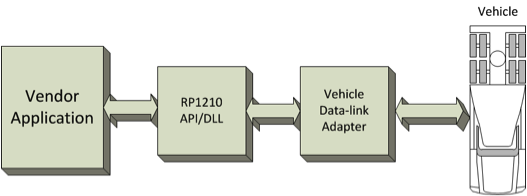
\includegraphics{RP1210}
  \caption{Diagram of RP1210 device and driver}
  \label{fig:rp1210}
\end{figure}

\subsection{RP1210 Functions and Their Uses}

A typical RP1210 session commences as follows. First, the file ``RP121032.INI'' is read to determine which RP1210-compliant devices are installed
on the system. When a device is chosen by the user, the appropriate DLL is loaded into memory and its exported functions are loaded into memory.
As the functions' names and prototypes are standardized, this process is vendor-agnostic.

Next, the client application calls the function \texttt{RP1210\_ClientConnect} to connect to the diagnostic link connector hardware. Assuming
the connection is successful, the client then issues one or more commands using the \texttt{RP1210\_SendCommand} function. This can filter incoming
messages based on MID or PGN, claim an address on a J1939 network, and other connection management functions. After the message filtering has been
set up, the client then uses \texttt{RP1210\_SendMessage} and \texttt{RP1210\_ReadMessage} to communicate on the network. The client terminates
the session with the \texttt{RP1210\_ClientDisconnect} call.

\section{Current Practices}

With the hardware and software requirements established, the typical procedure for an information download from heavy trucks can now be explained.
As mentioned previously, the information is typically downloaded using the engine manufacturer's diagnostic software. The normal use case
for diagnostic software is connecting to a diagnostic port in the cab of the truck using a diagnostic link connector, and accessing the desired
information with the maintenance software.

However, extracting crash information is not a normal use case. Because the truck has been in a high speed collision, the electrical connection
between the cab and the engine may have been severed, or the cab itself may be physically inaccessable. In these cases, the engine control module
must be removed and analyzed separately. This is performed either by placing the ECM in a donor vehicle identical to the one in the crash, or
by connecting to the ECM directly using the manufacturer's engine flashing harness. A bench download of a Cummins ECM is shown in figure \ref{fig:cumminsbench}.

Whatever method was used to connect to the ECM, the investigator then proceeds to extract the information using the manufacturer's diagnostic
software. This includes event data from the crash itself, mechanical fault information, engine tuning parameters, and driver behavior information.
This information is then recorded, in most cases, by printing the data to a PDF file. However, in many instances the software does not support
printing data and so it must be captured using a screenshot. All of the files resulting from the extraction are then stored on some kind of
removable media and produced to the client.

\subsection{For Contrast: Hard Disk Forensics}

In order to put current evidence handling practices for ECMs in the context of digital forensics in general, here the evidence extraction
procedures for hard disk drives is briefly explained. A more thorough treatment of this subject is given in \cite{carrier2005}.

Evidence disk drives are typically \emph{imaged}; that is, data is copied off the drive in the most raw form available from outside
the drive itself. The image is nothing more than a string of bits that have been copied sequentially from the disk drive. It includes
partition tables, filesystem metadata, deleted files, and more.

Devices called \emph{write blockers} are used to ensure the integrity of the evidence drive. They mediate the connection between the
drive and the computer that is imaging it, and any write commands originating from the computer are not forwarded on to the drive.
This prevents any accidental writes caused by investigator mistakes, automatic attempts by operating systems to mount file systems, etc.
Furthermore, the original disk is rarely accessed after the initial extraction, as all subsequent analysis is performed on the image.

To detect tampering or data corruption, the disk image is fingerprinted using a cryptographic hash function. This fingerprint is then recorded,
and can be verified later by re-hashing the image. Assuming that the hash itself can be protected, this re-hashing allows investigators to
detect any changes in the data.

\begin{figure}[h]

  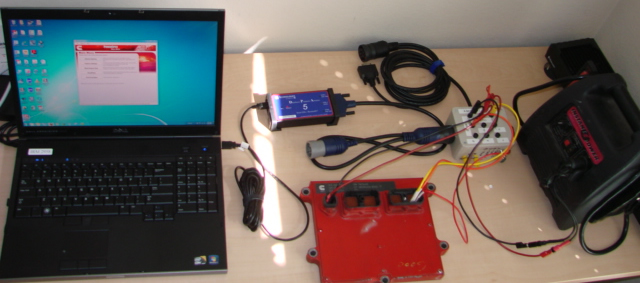
\includegraphics[scale=0.5]{cumminsbench}
  \caption{A bench download from a Cummins ECM}
  \label{fig:cumminsbench}
\end{figure}

\section{Forensic Soundness}

A heavy vehicle electronic control module (ECM) is a specialized process control computer that may have data of interest to an investigator. 
While ECMs may not have keyboards and monitors, they still are computers and have central processing units, memory, storage, and a means of 
networking or communicating with external devices. As such, many of the principles from computer forensics can be applied to heavy vehicle ECMs.

The first litmus test that any forensic methodology must pass is the rules of evidence for the legal system in which it is used. Here, we will
focus on the laws of the United States. The two primary standards to which evidence is held in that country are the Daubert standard, established
in the case \emph{Daubert v Merrell Dow Pharmaceuticals}, and the Federal Rules of Evidence. A review of the rules of evidence as they relate to 
digital forensics may be found in \cite{meyers2005}.

\begin{enumerate}
  \item Testimony must be relevant and reliable
  \item Judges have the task of ensuring that expert testimony rests on a reliable
        foundation and is relevant.
  \item Some or all of certain specific factors, including testing, peer review, error
        rates, and acceptibility in the relevant scientific community, may prove helpful
        in determining reliability of forensic testimony.
\end{enumerate}

\begin{enumerate}
  \item Method can be and has been tested
  \item Method has been subjected to peer review or publication.
  \item Method has a known error rate
\end{enumerate}

In addition to the general rules of evidence, the digital forensics literature contains many attempts to quantify the concept of forensic soundness.
A Special Report issued by the National Institute for Justice on Electronic Crime Scene Investigation \cite{NIJ2008} highlights the following basic forensic 
principles applied to dealing with digital evidence:

\begin{itemize}
\item Any process or procedure of collecting, transporting, or storing of digital evidence should not incur any changes to the evidence.
\item Only specifically trained experts should examine digital evidence.
\item Transparency during the operations of acquisition, transportation, and storage of the evidence should be maintained.
\end{itemize}

These basic tenets lay the foundation for the idea of forensic soundness. It is important to understand the term “forensically sound” 
as it relates to digital evidence. Many authors and professional organizations have attempted to rigorously define this concept, 
including the National Institute for Standards and Technology (NIST) \cite{NIST2001}, law enforcement entities such as the National Institute for 
Justice (NIJ) \cite{NIJ2008}, and academic bodies like the International Organization on Computer Evidence\cite{IOCE2002}. The methods of extracting, analyzing, 
and presenting digital evidence are forensically sound if they perform the task in a manner such that the results can be used in legal 
proceedings with a high degree of confidence in their admissibility. The process of extracting, interpreting, and presenting evidence 
will be referred to in this paper as the “forensic process.”

In addition to the NIJ report, McKemmish \cite{mckemmish2008} enumerates the following components of forensic soundness:

\begin{itemize}
\item \emph{Meaning} is a term that denotes confidence in the interpretation of extracted evidence data.
\item \emph{Error Detection} denotes processes for detecting or predicting errors in the forensic process.
\item \emph{Transparency} means the forensic process is documented, known, and verifiable.
\item \emph{Expertise} is required for those investigators examining digital data.
\end{itemize}

Casey \cite{casey2002} defines 7 levels of certainty for digital evidence that dictate how much weight should be given to the evidence in a case:

\begin{itemize}
\item C0: Evidence contradicts known facts
\item C1: Evidence is highly questionable.
\item C2: Only one source of evidence that is not protected against tampering
\item C3: Source(s) of evidence are more difficult to tamper with but there is insufficient evidence for a firm conclusion, or unexplained inconsistencies exist in available evidence
\item C4: Sole source evidence is protected against tampering or multiple, independent sources of evidence agree but the independent evidence is unprotected from tampering.
\item C5: Agreement of evidence from multiple, independent sources protected from tampering, but small uncertainties exist.
\item C6: The evidence is tamper proof and unquestionable.
\end{itemize}

While many of these levels include requirements that are encompassed by the requirements of error detection and certainty of meaning 
specified by McKemmish, this standard includes the principle of tamper resistance. In addition to protecting the evidence from tampering, 
we submit that a system which can demonstrate the absence of tampering also fulfills this requirement.

\section{Shortcomings of Current Practices}

Though several authors describe the concept of forensic soundness slightly differently, the basic concepts remain the same. The evidence must be extracted in a transparent,
repeatable, and verifiable manner that alters or destroys as little data as possible. There must be a high degree of certainty that the data is interpreted correctly. There must
be measures taken to ensure that the evidence has not been tampered with.

Unfortunately, current practices fail to meet these standards in several respects. First and foremost is that evidence extractions cannot be relied upon to leave the data unaltered.
Some engine maintainance software, by default, clears diagnostic fault codes after they are extracted from the engine. While this is desireable behavior for the software's typical
use case, in a forensic context it is unacceptable. In addition, if a bench download is being performed, the ECM is disconnected from all of the various sytems it was designed to monitor,
causing spurious fault codes to be created. With some manufacturers' products, especially Caterpillar, these can overwrite legitimate fault codes. The damage is made worse when
repeated downloads are conducted.

In addition to data extraction, current practices lack in the forensic soundness of the storage of data as well. No measures are taken to ensure that data have not been tampered
with. Data export formats, typically plaintext HTML or PDF documents, can easily be altered with readily-available software. Some manufacturers' native file formats are encrypted
somewhat, though not strongly: Cummins' EIF format is simply a password-protected ZIP archive, while Detroit Diesel's Drumroll files are encrypted using a simple XOR cipher.
Once decrypted, these files can be altered to remove evidence and re-encrypted easily.

Due to the potential for destruction of the source evidence and alteration of extracted data, it appears that current practice fails to pass the litmus test of forensic soundness
as currently accepted in the digital forensics community.

\chapter{Requirements of a Solution}

Regardless of the meaning of the digital data, it is necessary to present data in its final form in such a way that is transparent of its handling to establish trustworthiness. 
According to the transparency principle of forensic soundness, actions taken by an investigator should be available for later examination. Additionally, any error conditions 
encountered by the software should be recorded so that the legal weight of the evidence may be accurately considered. Audit trails are log files generated by forensic software 
to meet these requirements, and should at least be an option in any forensic solution.

\section{Baseline of Trust}

In order to make a full accounting of potential sources of error in any forensic process, it is important to examine the assumptions that the process requires. Standard methods of 
truck evidence extraction assume that the ECM is reporting data faithfully, that the vehicle network is accurately transmitting the communication to and from the ECM. It also assumes 
the Vehicle Diagnostic Adapter (VDA) is faithfully sending data from the vehicle network to the RP1210 library that is called by the OEM software.

While verifying the correct internal functioning of heavy truck ECMs is beyond the scope of this paper, the fidelity of data transmitted across the various networks (CAN bus, serial 
bus and USB) can be easily verified. Both protocols make use of error-correcting codes that detect transmission errors with very high reliability; for example, the CAN 
Cyclic Redundancy Check that is defined in the CAN standard process and detects all errors from 1 to 5 bits in the data frame, and only fails to detect 0.00018\% of 6-bit 
errors in a CAN frame\cite{koopman2004}. The represents a level of certainty that would take many years to experimentally verify because the likelihood of having an error and not knowing 
it is so low.

\section{Protocols}

Because typical ECM data extractions occur over vehicle networks, analysis of their forensic soundness requires knowledge of the protocols used for communication over those networks.

In heavy trucks, the networking protocols enumerate and define the various data that are transmitted over the in-vehicle network, which in turn provides clues as to the nature 
of the data present in the ECM. For example, a data type that is rounded to the nearest power of ten (186 rounded to 190, for example) when transmitted on the network might 
indicate that the value stored to and reported by the ECM is rounded in a similar fashion.

\section{Authentication}

A cryptographic hash function is an algorithm that generates a “fingerprint” of a given input. This fingerprint is generated in such a way that if a single bit of the input changes, 
roughly half the bits in the output file are altered\cite{schneier1996}. As such, they are commonly used to confirm that data have not been altered. A forensically sound tool should use a hash of 
the extracted truck evidence data to ensure that it has not been altered.

\section{Evidence Preservation}

Ideally, a forensic solution would allow the evidence to be preserved indefinitely. While hard disks are fairly inert when not used, heavy truck ECMs are actual computers that 
have some volatile data elements. One example is the ECM's system clock.

Some of the data on heavy truck ECMs is volatile, meaning that it requires a continuous supply of electrical power to avoid being deleted. One important example is the on-board 
system clock, which is important to investigators because it correlates with the timestamps associated with incident records. An exemplar circuit, shown in figure \ref{fig:clockbatt},is based around 
the EM Micro V3020, as used in several Detroit Diesel ECMs.  It is important that the actual on-board system clock be preserved, because the system clock is not necessarily synched 
up with standard times and the offset from the standard time must be recorded at the time of investigation.

Though the batteries in ECMs are large, and power drains slowly over time, this is an example of potentially critical information that can be lost if not extracted and preserved.

\begin{figure}[h]
  \centering
  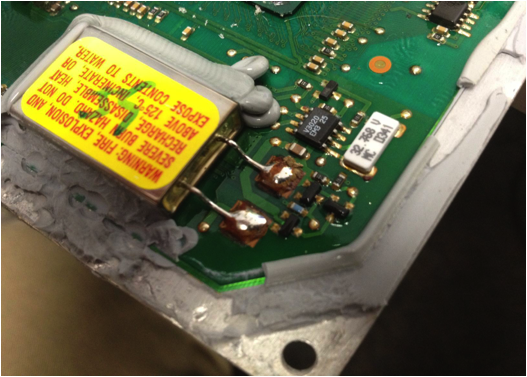
\includegraphics{clockbatt}
  \caption{The real time clock of a Detroit Diesel engine controller with system battery}
  \label{fig:clockbatt}

\end{figure}

\chapter{ECM Replay Software}

The solution arrived at was borrowed from the world of computer forensics. In a computer forensic investigation,
a low-level copy of the evidence drive is made; this copy is known as the ``disk image.'' Forensic analysis
is performed on this disk image instead of the original disk, so as to alter the original source evidence as
little as possible.

The goal was to extend this concept to truck ECMs: the information would be extracted exactly one time, and then
replayed upon further analysis. The replay traffic information would be stored securely to prevent malicious tampering
or accidental alteration.

\section{Software Requirements}

Development of the forensic replay software requires the following steps:

\begin{enumerate}
  \item Record the original information extraction process.
  \item Decipher any encryption or obfuscation mechanisms obscuring ECM data.
  \item Store the evidence in a secure manner.
  \item Respond to information requests identically to the ECM.
\end{enumerate}

All of these would ideally be performed in a manner that is as general as possible to minimize development time
supporting additional ECMs.

\section{Comparison of method to disk imaging}

The largest difference between the proposed extraction replay method and a forensic disk extraction is obviously
the amount of information extracted. When a disk is imaged, the entire physical contents of the disk (except for
any blocks hidden by a Dynamic Drive Overlay or a Host Protected Area) are extracted. However, a replay of a
software extraction only extracts the information normally accessed during that software extraction. It is possible
that some relevant information exists on the ECM that is not extracted.

Another difference is that protocols for accessing hard disks are standardized, so one method can be reasonably expected
to work reliably across all commercially available hard disks. ECMs, however, are acessed with proprietary protocols that
vary from manufacturer to manufacturer. Therefore, each individual manufacturer that will be supported requires the
reverse-engineering of that manufacturer's proprietary protocol extensions.

\section{Recording an extraction}

The first step in extracting data from an ECM was to determine how the manufacturers themselves extracted
the desired data. Without performing extensive static or dynamic analysis of the internals of the maintenance
software, it was determined that the best way to determine the extraction process was to record the messages
sent by the maintenance software to the ECM. Recording these messages could take place at two information boundaries,
the network or the diagnostic link connector driver.

\subsection{Network Recording}

Communication between the ECM and the maintenance software may be recorded at the network level, but this method
has some drawbacks.

First, recording traffic from the network requires additional hardware. In addition to the hardware normally required
to connect to ECMs, network recording requires some means of physically connecting to the network. Network-logging
hardware is also required. As it is not uncommon for ECM communications to take place over both J1708 and J1939, 
this hardware must be able to record both protocols.

Secondly, some meaning is lost. Applications typically use RP1210\_SendCommand calls to filter out broadcast communications
or other irrelevant messsages. Observation strictly at the network level does not provide any clues as to which messages
the application might be filtering, so important messages must be filtered out manually.

\subsection{RP1210 Recording}

An alternate method of recording information extraction is to record calls made to the RP1210 drivers
by the maintenance software. This had the advantage of not requiring additional hardware to 
record network traffic, and to abstract away the details of transport-layer operations of J1939.

Recording calls made to these RP1210 drivers was accomplished using a technique called API hooking\cite{Berdajs2010}.
A custom lightweight debugger was written using the PyDBG tool. Upon attaching the debugger to the software
in question, the debugger searches process memory for any loaded RP1210 drivers. Upon discovering a loaded RP1210
driver module, it places breakpoints on the following RP1210 function addresses:

\begin{enumerate}
  \item RP1210\_ReadMessage
  \item RP1210\_SendMessage
  \item RP1210\_ClientConnect
  \item RP1210\_SendCommand
  \item RP1210\_ClientDisconnect
\end{enumerate}

When execution hits one of these breakpoints, the debugger reads all arguments passed to the function when it was called,
and places a breakpoint on the function's return address so that return values can be read as well. In this way, all
messages sent to and received from the ECM are recorded by the debugging software.

This approach has a considerable advantage in that it doesn't require any additional hardware. Since the price of 
commercial vehicle network loggers can reach several hundred to several thousand dollars, cost-effectiveness should
not be overlooked. It also shows exactly which messages the application receives, which aids in determining which
messages are important. API hooking code is included in Appendix \ref{app:trace}.

\begin{figure}[h]
  \centering
  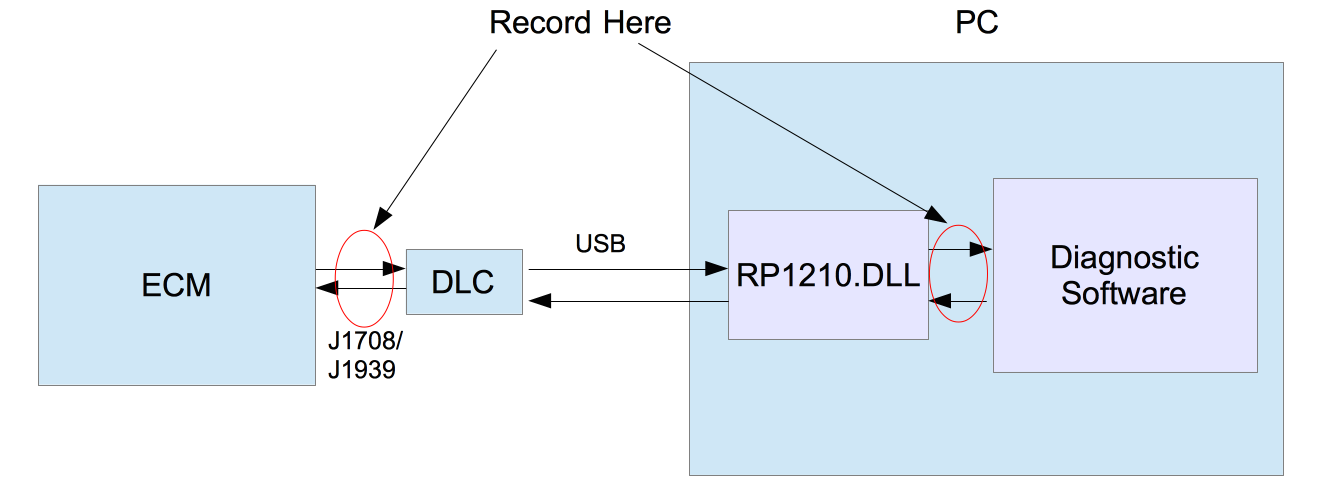
\includegraphics[scale=0.5]{RecordPoint}
  \caption{Information Boundaries for Recording}
  \label{fig:infoboundaries}
\end{figure}

\subsection{Recording Broadcast Data}



\section{Replaying an Extraction}

In order to ensure that the method of evidence extraction was as general as possible, evidence extraction was implemented
by simply replaying requests recorded during an actual information extraction. In the case of encrypted requests, where
the same request may be encrypted differently depending upon details of individual sessions, a transformation function
to decrypt the message and store it in a plaintext format needs to be specified.

After each request is replayed, responses to that request are recorded. The extraction data are stored as a list of 
key-value pairs, where the key is the request (transformed to a plaintext format, if applicable) and the value is
a list of all messages that the ECM sends in response to that request. This list is then serialized into a format
that can be stored in a file on disk; this file is the logical equivalent of a hard disk image.

As it has been observed that requests sent to the ECM may alter the state of the ECM, the replay mechanism must
be designed so that this is taken into account. The stored replay data are treated as a circular queue, with a current
index maintained during the extraction. Upon receipt of a message, the index is advanced until a matching response is found.
If responses to requests depend on earlier messages, receipt of the earlier messages will advance the index to
the expected response.

\subsection{Replaying Extracted Data}

Just as a transformation function may need to be specified for extraction of encrypted information, such a transformation
function may also need to be specified during replay. A comparison function needs to be specified, as the message format may
preclude the use of straight comparison of request data.

The solution arrived at uses two separate threads of control, one handling J1708/1587 communications and the other
handling J1939 communications. Each has its own protocol-specific response queue, though the two queues are both
stored in the same file for evidence storage and encryption.

\subsection{Replaying Broadcast Data}

\chapter{ECM Replay Hardware}


\section{Hardware Requirements}

While a computer connected to a diagnostic link connector can satisfactorily extract ECM data and replay
it to another computer running the diagnostic software, this setup is inconvenient for a number of reasons.
First of all, between the cost of a laptop computer and a diagnostic link connector, this cost of the setup
may reach into the thousands of dollars. Secondly, this equipment may be too cumbersome to carry into the field.
A different solution was required, and the following requirements were arrived at:

\begin{enumerate}
  \item The hardware must be inexpensive.
  \item It must be light and portable.
  \item It must be powerful enough to act as a general computing platform.
  \item It must be capable of communicating using heavy truck network protocols.
\end{enumerate}

\section{Hardware Platform}

\subsection{Computer Hardware}

The replay mechanism hardware is built around a BeagleBone, a commercially available ARM-based miniature computer produced
by Texas Instruments. The most recent iteration of the design, the BeagleBone Black, retails for roughly \$45 and has a 1GHz ARM
processor, 512MB of RAM, and 4GB of onboard flash storage. Weighing just a few ounces, it meets cost-effectiveness and portabilty
requirements.

\begin{figure}[h]
  \centering
  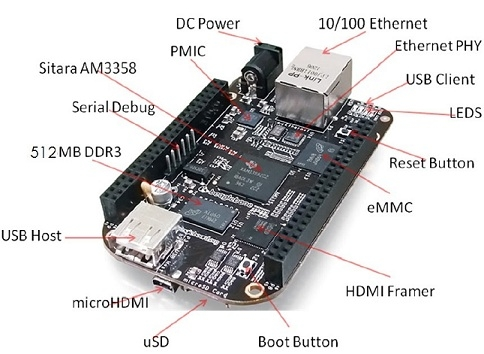
\includegraphics{BeagleBoneBlack}
  \caption{Beaglebone Black}
  \label{fig:BBB}
\end{figure}

\subsection{Capes}

One of the main reasons for adopting the BeagleBone platform is the capability to add functionality using expansion boards, known
as Capes. Commercially available capes include a RS-485 cape and a CAN cape, supporting the physical layers of J1708/J1587 and J1939
with little to no modification.


\begin{figure}[h]
  \centering
  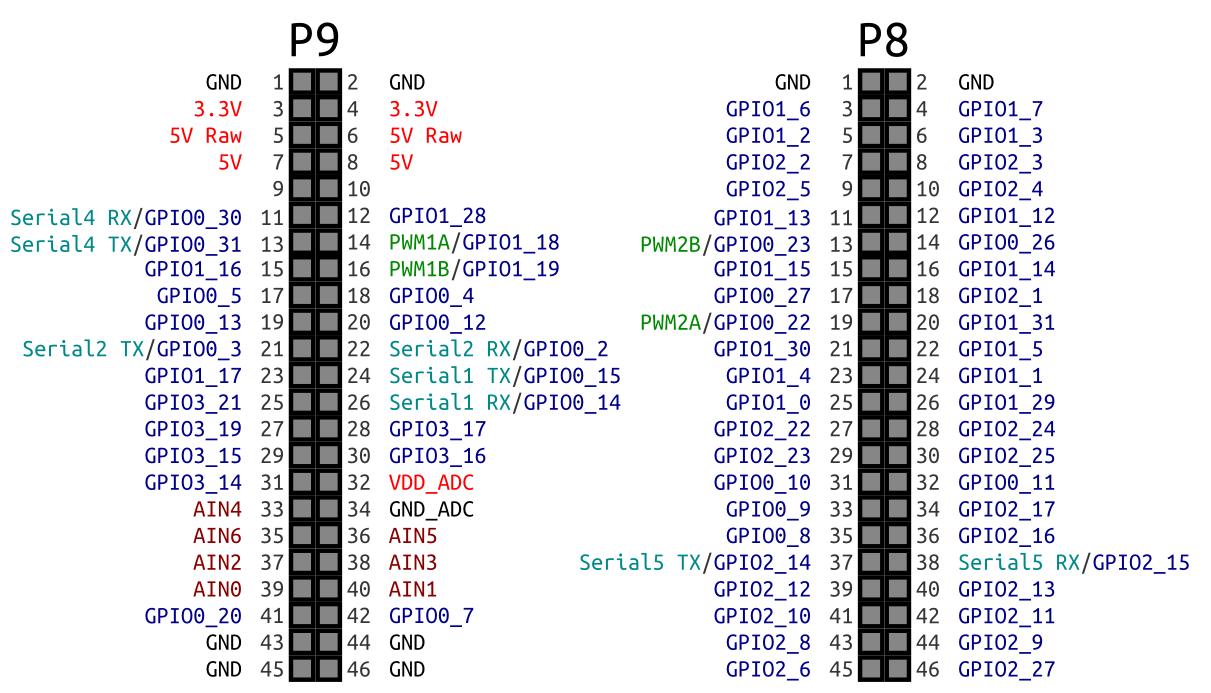
\includegraphics{BeaglebonePinout}
  \caption{Pinout of a Beaglebone Black}
  \label{fig:BBB-pinout}
\end{figure}

\section{Custom Cape}

As the currently available commercial options did not allow for communicating both over J1708 and J1939 networks, a custom
hardware solution was required. A custom cape was designed for heavy vehicle communications. A schematic is included in 
Appendex <include appendix label here>

The J1939 network interface required CAN transceiver hardware. The BeagleBone includes CAN hardware on the board, with access
to the module provided on pins <pins>. Likewise, the J1708/J1587 stack required J1708 hardware. An RS485 transceiver chip from TI
was wired up according to the specifications in the J1708 standard, and accessed through the BeagleBone's UART interface.

\subsection{Drivers}

Driver support for CAN was already well-documented in the BeagleBone; all that was required was to implement the J1939
functionality on top of it. An existing implementation of J1939 for the Linux kernel was found and compiled into
the BeagleBone's kernel as a module. As the remainder of the program was implemented in the Python programming language,
the Python socket module was also patched to work with J1939.

J1708 software drivers for Linux were nonexistent, so new drivers had to be written. Driver code is included in the
appendix.

\chapter{Case Study: Caterpillar}

The approach described in Chapter 3 was tested against ECMs manufactured by Caterpillar, Inc. This manufacturer was
chosen for several reasons. Firstly, the typical extraction process is long and tedious, and requires many screenshots to capture all the data. 
Secondly, as will be explained shortly, the proprietary communications protocol used
by Caterpillar is encrypted in such a way that implementing a replay mechanism is challenging.

\section{Caterpillar Data}

The information stored on the CAT ECMs under study include warranty report information and snapshot
information. The warranty report contains the identity of the ECM, historical usage information such as engine use histogram,
logged fault codes, and engine configuration information.

``Snapshots'' are a freeze-frame of the state of the truck at the time a critical fault is detected. These snapshots
include everything from wheel speed to engine speed. As a bench download can lead to new snapshots being created, overwriting
existing snapshot information, logging and replaying snapshot information is critical to any forensic solution for
Caterpillar ECMs.

\section{Deciphering Network Data}

Observation of RP1210 calls made by the Caterpillar ET software showed that all requests sent by,
and all responses to those requests, were made using extensions to the J1708/J1587 and J1939 protocols
proprietary to Caterpillar. As requests and responses changed significantly between extractions, with
no change in data displayed, it was determined that some session-based encryption mechanism was
used.

\subsection{Static Analysis}

As most of the CAT ET software is written using Microsoft's .NET framework, the software was decompiled
using JetBrains Software's dotPeek .NET decompiling tool. After some exploration of the code base,
the list of proprietary J1708 PIDs shown in Table \ref{tab:catet} was found.

\begin{table}[h]
  \centering
   \begin{tabular}{|c|c|}
    \hline
    Opcode & Function \\
    \hline
    0x70 & ReadRequest \\
    \hline
    0x80 & WriteRequest \\
    \hline
    0x90 & ReadWriteResponse\\
    \hline
    0xA0 & EncryptedBroadcastRequest\\
    \hline
    0xB0 & EncryptedBroadcastResponse\\
    \hline
    0xC0 & EncryptedReadRequest\\
    \hline
    0xD0 & EncryptedWriteRequest\\
    \hline
    0xE0 & EncryptedReadWriteResponse\\
    \hline
    0xF0 & SecuritySetup\\
    \hline
   \end{tabular}

\caption{Caterpillar ATA Function Codes}
\label{tab:catet}
\end{table}

The names of the functions obviously suggest that much of the message traffic is encrypted. Further analysis of the
decompiled code, and the disassembly of a native DLL,  revealed the following system:

\begin{enumerate}
  \item CAT ET sends a session key to the ECM using a SecuritySetup message.
  \item The ECM sends a session key to CAT ET using a SecuritySetup message.
  \item For each encrypted message, an individual key is generated by summing the
        current session key and the second nibble of the proprietary PID.
  \item Each message is passed to a native DLL along with its key for decryption.
  \item The key is an index into an array of bytes; the relevant byte is XOR'd
        with each byte in the message to encrypt/decrypt it.
\end{enumerate}


\begin{figure}[h]
  \centering
  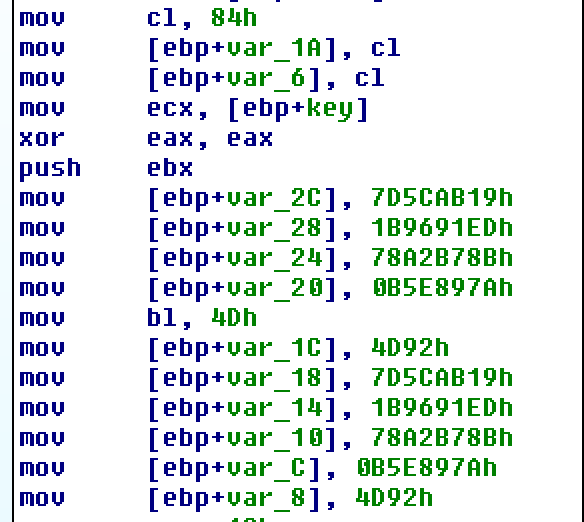
\includegraphics{CryptoKeysScreenshot}
  \caption{Disassembly showing decryption/encryption keys}
  \label{fig:atacryptkeys}
\end{figure}

\begin{figure}[h]
  \centering
  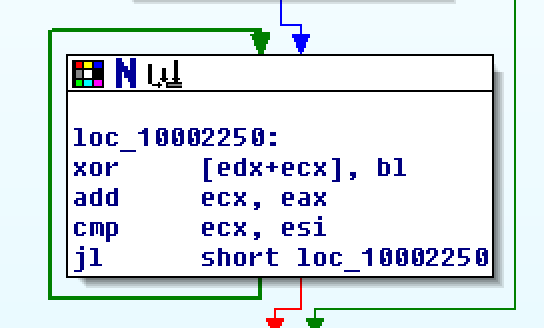
\includegraphics{CryptoAlgorithmScreenshot}
  \caption{Dissasembly showing decryption/encryption process}
  \label{fig:atacryptalgorithm}
\end{figure}


\subsection{Dynamic Analysis}

Now that the algorithm that encrypted ECM communications was known, the information contained in those
messages could be observed to determine how that information should be extracted and replayed. The
API hooking tool described in Chapter 3 was extended to decrypt ECM communications on-the-fly
and log them when they were intercepted. It was discovered that the protocols followed the format depicted
in Figure \ref{fig:ataprotocol}

\begin{figure}[h]
  \centering
  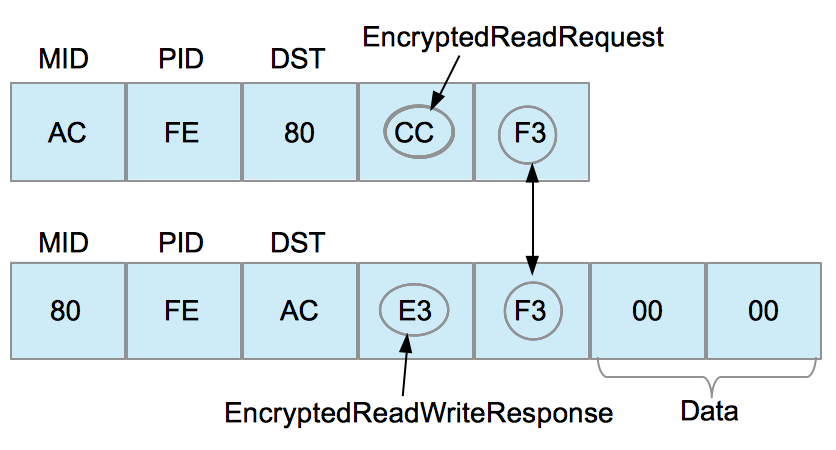
\includegraphics{cat-protocol-diagram}
  \caption{Example exchange in CAT ATA protocol}
  \label{fig:ataprotocol}
\end{figure}

\section{Information Extraction}

Now that the mechanism of the protocol was somewhat understood, it was possible to extract the information.
A manual extraction was performed according to a checklist for a crash information extraction, and the 
RP1210 API calls were logged.

Each request was logged in a plaintext format as it was sent. 
It should be noted that the storage format preserves the opcode of the message. After the message was sent, proprietary
responses with matching PIDs were recorded in the key-value pair. It was observed that some responses were split over
several messages, so this was accounted for in the extraction software.

\section{Verification}

In order to ensure that the method of information extraction was reliable, replays from the ECM were tested against
actual extractions from CAT ECMs.

\subsection{Procedure}

The ECMs tested were evidence ECMs that were already used, and thus had been pre-populated with data.
The verification procedure was designed to determine the fidelity of the information replayed, as well as the
consistency of multiple replays of recorded data as compared to the consistency of multiple downloads of an
evidence ECM. The test procedure also aimed to test the generality of the specific ECM replay method derived
for Caterpillar ECMs by performing the same test against multiple ECMs.

\begin{figure}[h]
  \centering
  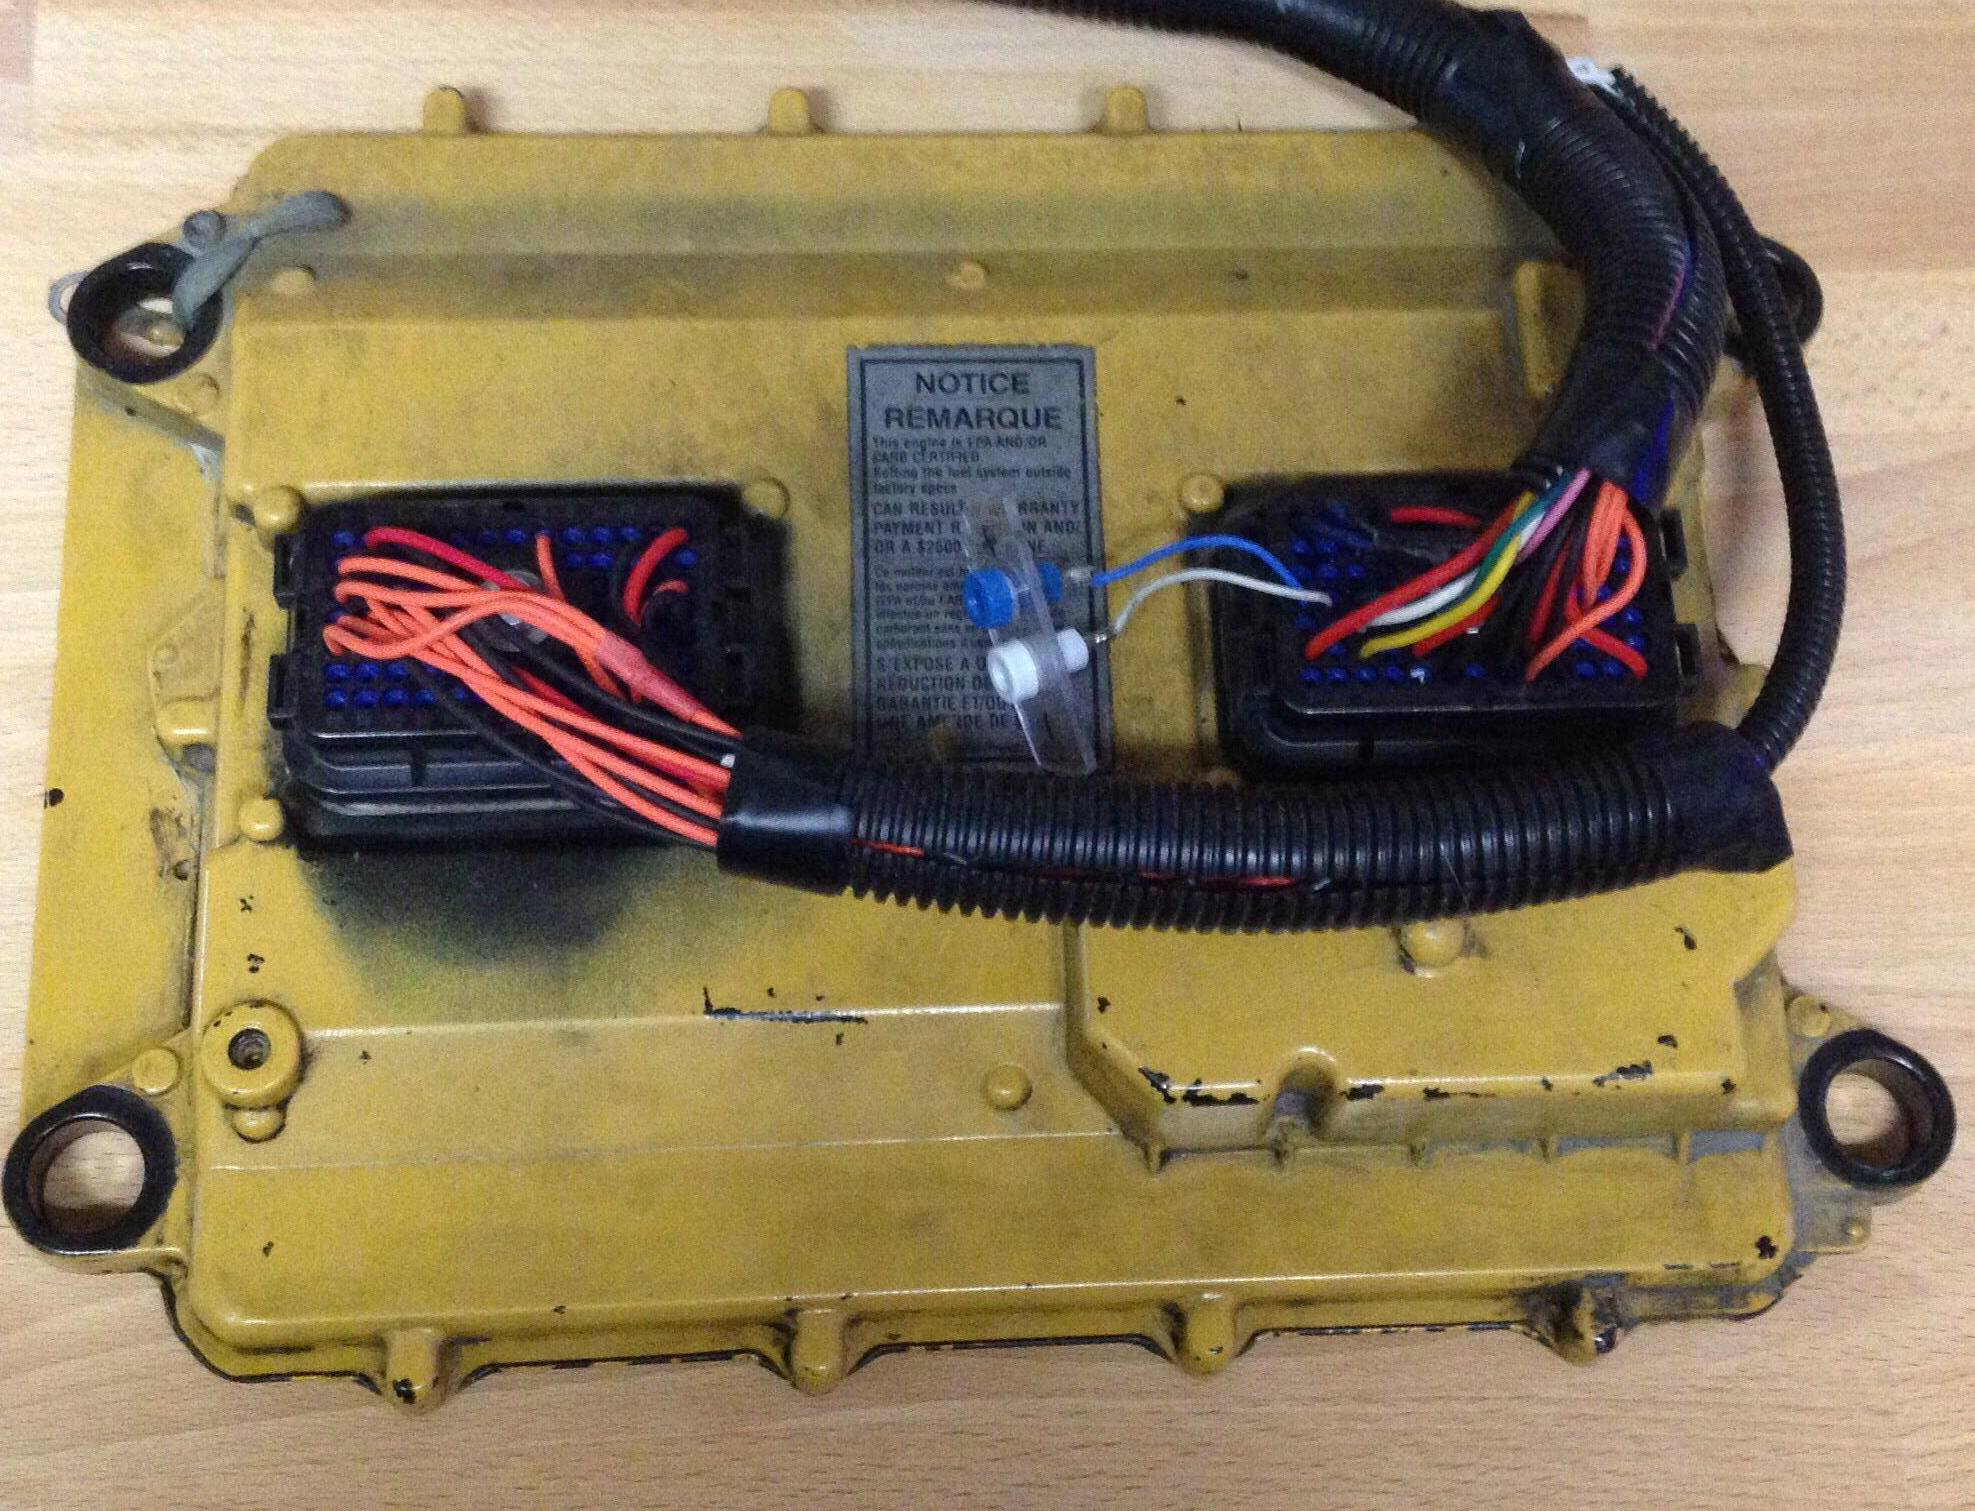
\includegraphics[scale=.2]{cat-ecm-1}
  \caption{First ECM for which replay was developed.}
  \label{fig:cat-ecm-1}
\end{figure}

\begin{figure}[h]
  \centering
  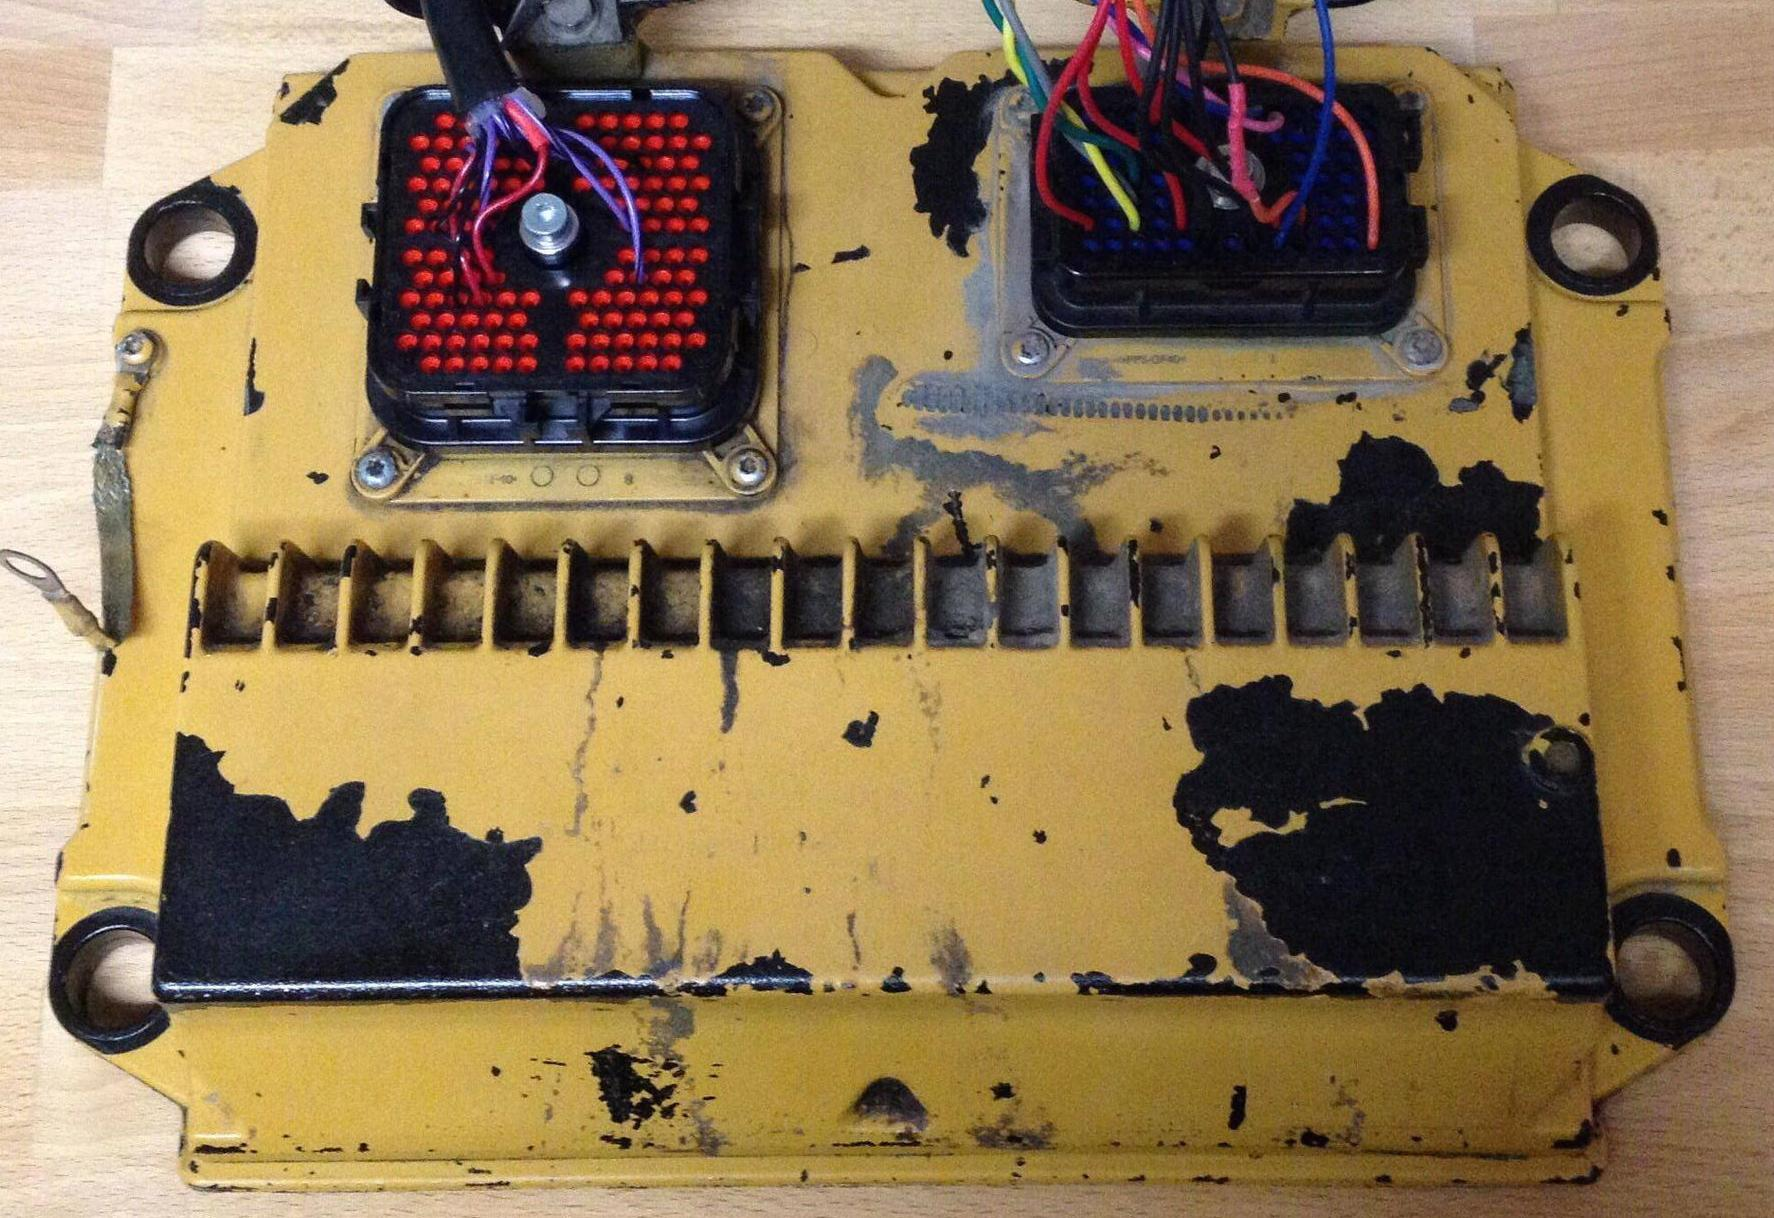
\includegraphics[scale=.2]{cat-ecm-2}
  \caption{Second test ECM, a CAT ADEM IV}
  \label{fig:cat-ecm-2}
\end{figure}


The steps of the test procedure were as follows:

\begin{enumerate}
  \item Perform one extraction of test ECM according to checklist while recording API calls. Save Warranty Report information and record snapshot information.
  \item Repeat step one twice more, each time saving Warranty Reports and recording snapshots.
  \item Extract ECM data using logged RP1210 calls obtained in step 1.
  \item Perform 3 replayed extractions, using data extracted in step 3.
  \item Compare ECM extractions to find differences in data contained therein.
  \item Compare replayed extractions to find differences in data.
  \item Compare consistency of ECM extractions and replayed extractions.
\end{enumerate}

As snapshot data can be recorded manually, these comparisons were carried out by hand. Warranty report information, however,
is stored in a plain-text XML format. Accordingly, the data contained in these files could be compared using a suite of tools developed
by Adrian Mouat\cite{Mouat2002} for XML comparison.

\subsection{Results}


\chapter{Cryptographic Protection}

To maximally ensure the data extracted are protected from alteration,
they needed some form of cryptographic protection that would make it impossible, or at
least very unlikely, that the evidence could be altered in a manner that would not be
detected. The protection requirements are as follows:

\begin{enumerate}
  \item The data must be protected from alteration
  \item The data must be protected despite the fact that all computation takes
        place on a device that is solely within the control of an unknown person.
  \item Others' data must be secure even if a single device is compromised.

\end{enumerate}

\section{Protection Mechanism}

In traditional computer forensic investigations, a disk image is protected by performing
a cryptographic hash on it. Later on, the image is hashed again and the two hashes are compared
to confirm that the image has not changed. The disk imaging process frequently takes place in an
office, where all parties involved in the case can easily be present to ensure that the extraction
is performed properly and no data are altered.

In the case of ECM data records, however, the use case is somewhat different. The data are frequently
extracted in remote locations where it is not feasible to have all parties to the case present. Therefore,
the individual extracting the information has total access to the information being extracted, likely for
a significant length of time. In this case, hashing alone may not offer the required protection as the data
may just be altered and the hash recomputed. While this is also a risk in hard drive extractions, the possibility
of having all parties present mitigates that somewhat.

Rather than attempting to protect the data from alteration, which is practically impossible with the device
in the physical control of a potentially malicious actor, the solution is to strongly encrypt
the data instead. If the data are strongly encrypted, while altering the data may be possible, 
\emph{meaningfully} altering the data is impossible. By ensuring that an attacker will gain nothing by
altering the data, the data are effectively prevented from being altered.

\section{Cryptosystem}

While strongly encrypting the data protects it from alteration, encrypting the data on a remote device in such
a way that the key is not discovered is a non-trivial exercise. The following encryption algorithm was developed
to perform this task:

\begin{enumerate}
  \item A nonce, to be used as a symmetric key, is randomly generated.
  \item The nonce is used to encrypt the data.
  \item A public key, stored on the device, is used to encrypt the key.
  \item The encrypted key is stored alongside the encrypted disk image.
  \item Later, the RSA private key, stored with a trusted third party, is
        used to decrypt the symmetric key, which is then used to decrypt
        the data.
\end{enumerate}

This is an example of a hybrid cryptosystem as described in \cite{cramer2004}. Cramer and Shoup prove that a hybrid cryptosystem of
this type is secure so long as the underlying algorithms are secure, and the padding scheme used for encrypting the key is secure.

\section{Cryptosystem Implementation}

While the general cryptosystem is agnostic in terms of the actual algorithms used, a practical implementation requires specific
algorithms to be chosen.

The symmetric algorithm chosen to protect the data is AES-128, as the AES algorithm is the industry standard symmetric encryption
algorithm, and it is currently believed to be secure. The 128-bit key length was chosen because of breaks discovered in the 256-bit
key length\cite{Biryukov2009}.

The cryptographic hash function chosen is SHA-256. While a longer hash value may yield better security, a longer hash may also make
it more difficult to write down a hash value for an investigator in the field. SHA-2 was chosen over SHA-1 because of the widely-published
attacks on SHA-1\cite{Manuel2011}.

In keeping with current security best practices, the symmetric keys are padded according to the PKCS\#1-OAEP standard before encryption\cite{Bellare1995}.


\chapter{Conclusions and Future Work}

\section{Summary of Provided Solution}

As can be seen from the diffs of Warranty Files from the various extractions, replayed data is consistent with
traditionally extracted data in all respects, and is in fact more consistent in some areas.

\subsection{Forensic Soundness}


The NIJ and McKemmish both address forensic soundness, though their approaches are similar enough to be
treated together.

The NIJ's definition of forensic soundness has three elements:

\begin{enumerate}
  \item Any process or procedure of collecting, transporting, or storing of digital evidence should not incur any changes to the evidence.
  \item Only specifically trained experts should examine digital evidence.
  \item Transparency during the operations of acquisition, transportation, and storage of the evidence should be maintained.
\end{enumerate}

McKemmish's similar definition has four:

\begin{itemize}
\item \emph{Meaning} is a term that denotes confidence in the interpretation of extracted evidence data.
\item \emph{Error Detection} denotes processes for detecting or predicting errors in the forensic process.
\item \emph{Transparency} means the forensic process is documented, known, and verifiable.
\item \emph{Expertise} is required for those investigators examining digital data.
\end{itemize}

As can be seen from the verification results, the original evidence is modified less using forensic replay than it is by repeatedly
extracting the information by traditional means. Even if no additional faults are created during a bench download, the ECM running
time is better preserved by imaging and replaying the ECM data rather than repeated downloads.

The expertise requirement is not totally alleviated by the extraction and replay process; an investigator still has to know how to 
connect to the ECM and power it up properly. However, the main advantage of the forensic extraction and replay process is that
all information extraction is automated; no knowledge of diagnostic software or the steps required to gather pertinent crash information
is needed. This is an advantage in a law enforcement context where training time is at a premium.

By default, the CAT ECM extraction process is almost completely opaque. Unless certain data are not available on the ECM, or an error
occurs during the download process, there is no record kept of the traffic other than its final interpretation by the maintenance
software. As the forensic replay method is literally a recording of network traffic, this traffic can be examined after the fact
to verify the extraction and replay process.

Eoghan Casey's definition of forensic soundness includes seven levels of forensic certainty based on certain characteristics
of the evidence and the method in which it is stored:

\begin{itemize}
\item C0: Evidence contradicts known facts
\item C1: Evidence is highly questionable.
\item C2: Only one source of evidence that is not protected against tampering
\item C3: Source(s) of evidence are more difficult to tamper with but there is insufficient evidence for a firm conclusion, or unexplained inconsistencies exist in available evidence
\item C4: Sole source evidence is protected against tampering or multiple, independent sources of evidence agree but the independent evidence is unprotected from tampering.
\item C5: Agreement of evidence from multiple, independent sources protected from tampering, but small uncertainties exist.
\item C6: The evidence is tamper proof and unquestionable.
\end{itemize}

The solution outlined herein makes no claim about the veracity of the evidence as it relates to physical phenomena, except that it is a faithful representation of the information communicated
by the ECM, but the other characteristics of evidence can be compared. The main difference here is that when extracting and storing evidence through traditional means, even if the
evidence agrees with other sources it is not tamper-proof, and thus can only achieve a rating of C4 in the absolute best case (i.e. there is physical evidence corroborating the 
digital evidence). However, with the tamper protections added by the cryptosystem presented herein, the digital evidence is rated at C4 at bare minimum, reaching C5 or C6 with corroborating
physical evidence. 

\subsection{Practicality}

Currently, in order to perform an evidence download from a heavy vehicle ECM, investigators require at bare minimum a laptop and a diagnostic link connector.
If a bench download is to be performed, an engine flashing harness is required as well. Unfortunately, removing the need for an engine flashing harness is
beyond the scope of this work. However, this replay solution represents a logistical advantage over existing methods.

While the current use case still requires a laptop, it does not require any software beyond a simple web browser. This greatly simplifies software logistics, as well
as reducing the cost of software required to conduct investigations in the field. The hardware can be made no larger or heavier than existing diagnostic link connectors
while remaining far cheaper.

\section{Future Work}

\subsection{Understanding Meaning}

The current solution requires that investigators use the manufacturers' maintenance software to interpret the data that has been extracted and replayed from the ECM.
While this is an improvement over the current situation in terms of ease and practicality, it is also not ideal. Future work in this area should include analyzing the
meaning of the extracted ECM data, so that it can be analyzed and presented independently of proprietary software.

\subsection{Information Verification}

New work might also include verification of the interpretation of the data. Currently, it is assumed that the data reported by the ECM accurately reflect the conditions
observed during incidents, and that the manufacturers' software accurately interprets this reported data. 

% LocalWords:  ics


%%%%%%%%%%%%%%%%%%%%%%%%%%%%%%%%%
% BIBLIOGRAPHY
%%%%%%%%%%%%%%%%%%%%%%%%%%%%%%%%%

%\addtocontents{toc}{\protect{\hfill \ }}
%\addcontentsline{toc}{section}{\contentsadj NOMENCLATURE}

\bibliographyp
\bibliography{jj-phd-proposal}
\bibliographystyle{unsrt}

%%%%%%%%%%%%%%%%%%%%%%%%%%%%%%%%%
% APPENDICES AS NECESSARY
%%%%%%%%%%%%%%%%%%%%%%%%%%%%%%%%%
\addcontentsline{toc}{chapter}{\protect\numberline{}{Appendices}}
\appendixpages       % prepare for the generation of the appendices

%\begin{appendices}
\TUappendix{Code Listings}\label{app:code}

\TUsection{Extraction Code}

\TUsubsection{catextract.py}\label{app:extraction}
%\lstset{basicstyle=\small}
%\lstinputlisting[language=Python]{catreplay/simple-extract.py}
\begin{minted}{python}
import RP1210
import logfileparser
import sys
from RP1210Defines import *
import catATA
import time
import ATAClient
import atamessage
import pickle
import J1587_Transport as transport
import responses as response_utils
#import threading


excluded_pids = [[0xfc,0x58]]
multiple_pids = {0xDB:8,0xD3:10}


dupefile = open("dupefile.txt","w")
def get_proprietary(driver):
   start = time.time()
   while True:
      if time.time() - start > 2:
         print("timed out while waiting for response")
         return None
      msg = driver.read_message()
      if len(msg) < 5:
         continue
      if catATA.is_proprietary(msg) or msg[1] == 0xc5:
#         print(msg[4:])
         return msg
      else:
         continue

def get_num_responses(pid):
   if pid in excluded_pids:
      return 0
   elif pid in multiple_pids.keys():
      return multiple_pids[pid]
   else:
      return 1

def get_pid_msg(msg,key,driver):
   got_pid = False
   this_pid = msg.pid
   start = time.time()
   retmsg = None
   while (not got_pid) and (not time.time() - start > 5):
      inbuf = get_proprietary(driver)
      if inbuf is None:
         #driver.send_message(msg.to_buffer())
         continue

      elif inbuf[1] == 0xc5:
         print("transport protocol engage")
         tmp = transport.receive_message(msg.src,msg.dst,driver,rts=inbuf)#check these src dst assignments if there's problems
         if tmp[0] == 0xfe:
            retmsg = atamessage.ATAMessage.from_transport(msg.dst,msg.src,tmp,key=key)
            print("I think the PID is %d, hoping for %d" % (retmsg.pid,this_pid))
      else:
         retmsg = atamessage.ATAMessage.from_buf(inbuf,key=key)
         print("I think the PID is %d, hoping for %d" % (retmsg.pid,this_pid))

      if retmsg.pid == this_pid:
         got_pid = True
      else:
         retmsg = None

   return retmsg



def get_pid(msg,key,driver):
   if msg.data in excluded_pids:
      return []
   pid = msg.pid
   responses = []
   numresponses = get_num_responses(pid)
   i = 0
   tries = 0
   if numresponses > 1:
      dupefile.write("\n\n")
   while i < numresponses:
      respmsg = get_pid_msg(msg,key,driver)

      if respmsg is not None:
         dupe = False
         for r in responses:
            if response_utils.compare_J1708_msg(respmsg.to_plain_buffer(),r.to_plain_buffer()):
               dupe = True
               break
         if dupe:
            continue
         responses.append(respmsg)
         i += 1
      else:
         i = 0
         driver.send_message(msg.to_buffer())
   if len(responses) > 1:
      for r in responses:
         dupefile.write(str(r.to_plain_buffer()))
   return responses





def get_setup(msg,driver):
   setup = False
   while not setup:
      inmsg = get_proprietary(j1708)
      if inmsg is None:
         driver.send_message(msg)
         continue
      if inmsg[1] == 0xc5:
         continue
      thismsg = atamessage.ATAMessage.from_buf(inmsg)
      if thismsg.is_setup():
         return thismsg.data[-1] & 0x0F
      else:
         continue


def get_encrypted_response(driver):
   return get_command(driver,[0xB0,0xC0])

def get_unencrypted_response(driver):
   return get_command(driver,[0x90])

def get_encryption_setup(driver):
   return get_command(driver,[0xF0])


   


driver = RP1210.RP1210Driver("DPA4PMA.DLL")
driver.initialize()


try:
   fh = open(sys.argv[1],"r")
except:
   print(sys.argv[1])
   print("error opening file")
   sys.exit(-1)
   
tokens = logfileparser.tokenize_file(fh)

   
tdriver = RP1210.RP1210Driver("DPA4PMA.DLL")
tdriver.initialize()
j1708 = RP1210.J1708_Provider("DPA4PMA.DLL",driver=tdriver)
j1939 = RP1210.J1939_Provider("DPA4PMA.DLL",driver=tdriver)
j1708.initialize()
j1939.initialize()

print("all set up, press any key to start extracting.")

sys.stdin.read(1)
ataclient = ATAClient.ATAClient(j1708)
protocols = {}
J1708ResponseQueue = []
J1939ResponseQueue = []
for i in range(len(tokens)):
   token = tokens[i]
   buf = token.split(",")
   
   if buf[1] == "SC" or buf[1] == "CD":
      continue
   elif buf[1] == "CC" and buf[2] == "00":
      protocols[buf[3]] = buf[5]
   elif buf[1] == "SM":
      #print(buf)
      msg = logfileparser.send_message(token,proto=protocols[buf[0]])
      if protocols[buf[0]] == "J1708":
         if len(msg.data) < 5 or not msg.data[1] == 0xFE:
            continue
         j1708.send_message(msg.data)
         sm = atamessage.ATAMessage.from_buf(msg.data,key=ataclient.encrypt_key)
         if sm.is_setup():
            ataclient.encrypt_key = sm.data[-1] & 0x0F
            ataclient.decrypt_key = get_setup(msg.data,j1708)
            print("encrypt key: %d decrypt key: %d" % (ataclient.encrypt_key,ataclient.decrypt_key))
         else:
            print("Trying to match %s" % sm.to_plain_buffer())
            responses = get_pid(sm,ataclient.decrypt_key,j1708)
            if len(responses) > 0:
               thisqueue = []
               for response in responses:
                  thisqueue.append(response.to_plain_buffer())
               J1708ResponseQueue.append([sm.to_plain_buffer(),thisqueue])
               print(J1708ResponseQueue[-1])

         time.sleep(.3)

         
      elif protocols[buf[0]] == "J1939":
         #msg = logfileparser.send_message(token,proto=protocols[buf[0]])
         j1939.send_raw(msg.data)
#         time.sleep(.3)
#         print("j1939 sent: %s" % msg.data)
         inmsg = j1939.read_raw()
         while len(inmsg) == 0:
            j1939.send_raw(msg.data)
            inmsg = j1939.read_raw()

         J1939ResponseQueue.append([msg.data,inmsg])
         print(J1939ResponseQueue[-1])
         time.sleep(.3)

      
      #driver.send_message(msg.client_id,msg.data)
      #just send this message.
   else:
      pass

del(j1708)
del(j1939)
fh.close()

#fh2 = open("responses2.txt","w")

#for response in ataclient.J1708responses:
#   fh2.write("%s   %s\n" % (list(map(hex,response[0].to_plain_buffer())),list(map(hex,response[1].to_plain_buffer()))))

#fh2.close()

try:
   queues = (J1708ResponseQueue,J1939ResponseQueue)
   response_queues = open("responsequeues.pkl","wb")
   pickle.dump(queues,response_queues)
   response_queues.close()
except:
   print("Problem pickling responses")


print("Extraction complete!\a\a\a\a")
\end{minted}

\TUsubsection{catreplay.py}\label{app:replay}
\begin{minted}{python}
import RP1210
import logfileparser
import sys
from RP1210Defines import *
import catATA
import time
import ATAClient
import atamessage
import pickle
from multiprocessing import Process
from responses import ResponseQueue
import J1587_Transport as transport
#import threading

encrypt_key = None
decrypt_key = None

'''tdriver = RP1210.RP1210Driver("DPA4PMA.DLL")
tdriver.initialize()

j1939 = RP1210.J1939_Provider("DPA4PMA.DLL",driver=tdriver)
j1708.initialize()
j1939.initialize()'''

def j1708_replay_callback(recvd_msg,resp_queue):
  global encrypt_key
  global decrypt_key
  if not atamessage.is_proprietary(recvd_msg):
    return
  if len(recvd_msg) < 5:
    return
  inmessage = atamessage.ATAMessage.from_buf(recvd_msg,key=decrypt_key)
  to_send = []
  if inmessage.is_setup():
    #print("setting decrypt key to %d" % (inmessage.data[-1] & 0x0F))
    decrypt_key = inmessage.data[-1] & 0x0F
    to_send.append(atamessage.ATAMessage(0x80,0xAC,atamessage.SECURITY_SETUP,[0x0B]))
    encrypt_key = 0x0B & 0x0F
    return to_send
  else:
    #print("Received: %s" % list(map(hex,inmessage.to_plain_buffer())))
    to_send_raw = resp_queue.get_j1708(inmessage.to_plain_buffer())
    if to_send_raw is not None and len(to_send_raw) > 0:
      for tsr in to_send_raw:
        to_send.append(atamessage.ATAMessage.from_plain_buf(tsr,key=encrypt_key))
        if len(to_send_raw) > 1:
          print("Sending: %s" % list(map(hex,tsr)))
      return to_send
    else:
      return None

def j1939_replay_callback(recvd_msg,resp_queue):
  outmsg = resp_queue.get_j1939(recvd_msg)
  return outmsg

def j1708_replay_proc(resp_queue):
#  tdriver = RP1210.RP1210Driver("DPA4PMA.DLL")
#  tdriver.initialize()
  driver = RP1210.J1708_Provider("DPA4PMA.DLL")
  driver.initialize()
  while True:
    inmsg = driver.read_message()
    outmsg_list = j1708_replay_callback(inmsg,resp_queue)
    if outmsg_list is None or len(outmsg_list) == 0:
      print("no outmsgs, continuing")
      continue
    else:
      for outmsg in outmsg_list:
        #print("sending %s" % outmsg)
        time.sleep(.05)
        if len(outmsg.data) + 2 <= 21:
          driver.send_message(outmsg.to_buffer())
        else:
          (src,dst,data) = outmsg.to_transport()
          transport.send_message(src,dst,data,driver)


def j1939_replay_proc(resp_queue):
  #tdriver = RP1210.RP1210Driver("DPA4PMA.DLL")
  #tdriver.initialize()
  driver = RP1210.J1939_Provider("DPA4PMA.DLL")
  driver.initialize()
  while True:
    inmsg = driver.read_raw()
    print("J1939 Received: %s" % list(map(hex,inmsg)))
    outmsg = j1939_replay_callback(inmsg,resp_queue)
    if outmsg:
      driver.send_raw(outmsg)


if __name__ == '__main__':
  try:
    queuesfh = open("responsequeues.pkl","rb")
    queues = pickle.load(queuesfh)
  except:
    print("Could not load response queues.")
    sys.exit(1)

  j1708_queue = queues[0]
  
  j1939_queue = queues[1]

  resp_queue = ResponseQueue(J1708requests=j1708_queue,J1939requests=j1939_queue)

  print("all set up, press any key to start replay.")
  sys.stdin.read(1)

  j1708process = Process(target=j1708_replay_proc,args=(resp_queue,))
  j1939process = Process(target=j1939_replay_proc,args=(resp_queue,))

  j1708process.start()
  j1939process.start()

  while True:
    q = sys.stdin.read(1)
    if q == "q":
      j1708process.terminate()
      j1939process.terminate()
      sys.exit(1)




\end{minted}

\TUsubsection{logfileparser.py}
\begin{minted}{python}
import re
import sys


#matches the beginning of a message but not a wrapped-around message
token = re.compile('(\d\d|XX),(CC|CD|SM|SC|RM).*')
fragment = re.compile('(\S\S,?)+$')
messages = []

class rp1210_client():
  def __init__(self,client_id,flags):
    self.client_id = client_id
    self.flags = flags

def tokenize_file(fh):
  lines = fh.readlines()
  tokens = []
  for line in lines:
    mymatch = token.search(line)
    if mymatch:
      tokens.append(mymatch.group(0))
    else:
      newmatch = fragment.search(line)
      tokens[-1] += newmatch.group(0)
  
  for i in range(len(tokens)):
    if tokens[i][-1] == ",":
      tokens[i] = tokens[i][:-1]
      
  return tokens
  
class rp1210_msg():
  def __init__(self,tokenstring):
    self.dat = tokenstring.split(",")
    self.message_type = self.dat[1]
    
class client_connect(rp1210_msg):
  def __init__(self,tokenstring):
    super().__init__(tokenstring)
    self.client_id = int(self.dat[3])
    self.protocol = self.dat[5]
    #This should be enough. I don't think we need to know Tx/Rx buffer sizes 
    
class send_command(rp1210_msg):
  def __init__(self,tokenstring):
    super().__init__(tokenstring)
    self.client_id = int(self.dat[0])
    self.retval = int(self.dat[2])
    self.msg_size = int(self.dat[3])
    self.command_number = int(self.dat[4])
    if self.msg_size > 0:
      self.msg_string = list(map(lambda x: chr(int(x,16)),self.dat[5:]))
    else:
      self.msg_string = ""
    
class send_message(rp1210_msg):
  def __init__(self,tokenstring,proto="J1939"):
    super().__init__(tokenstring)
    self.client_id = int(self.dat[0])
    self.bytes_sent = int(self.dat[3])
    if proto == "J1708":#Account for the first byte in the buffer being the priority byte.
      self.data = list(map(lambda x: int(x,16),self.dat[7:]))
    else:
      self.data = list(map(lambda x: int(x,16),self.dat[6:]))
    
#note: track client_connect calls to see if need to account for echo byte
class read_message(rp1210_msg):
  def __init__(self,tokenstring):
    super().__init__(tokenstring)
    self.client_id = int(self.dat[0])
    self.bytes_received = int(self.dat[2])
    self.timestamp = int("".join(self.dat[5:9]),16)
    self.data = list(map(lambda x: int(x,16),self.dat[9:]))
  
if __name__ == "__main__":
  filename = sys.argv[1]
  try:
    fh = open(filename,'r')
  except:
    print("problem reading file")
    sys.exit(1)
    
  tokenlist = tokenize_file(fh)
      
  for a in tokenlist:
    print(a)
    




\end{minted}

\TUsubsection{ATAClient.py}
\begin{minted}{python}

import atamessage
import J1587_Transport as transport
import copy


class j1939holder():
  def __init__(self,indata):
    self.data = indata
  def to_plain_buffer(self):
    return self.data

class ATAClient():
  def __init__(self,driver,J1708responses=None,J1939responses=None):
    self.driver = driver
    self.encrypt_key = None
    self.decrypt_key = None
    self.src = 0xAC
    if J1708responses is None:
      self.J1708responses = []
    if J1939responses is None:
      self.J1939responses = []

  #callback for when extractions are performed
  def extraction_callback(self,sent_msg,recvd_msgs):
    outmessage = atamessage.ATAMessage.from_buf(sent_msg,key=self.encrypt_key)
    print("Sent: %s" % list(map(hex,sent_msg)))
    this_queue = []
    for recvd_msg in recvd_msgs:
      if atamessage.is_proprietary(recvd_msg):
        print("Received: %s" % list(map(hex,recvd_msg)))
        inmessage = atamessage.ATAMessage.from_buf(recvd_msg,key=self.decrypt_key)
        if inmessage.is_setup():
          print(list(map(hex,recvd_msg)))
          print("setting decrypt key to %d" % (inmessage.data[-1] & 0x0F))
          self.decrypt_key = inmessage.data[-1] & 0x0F
        else:
          this_queue.append(inmessage.to_plain_buffer())
        #self.J1708responses.append((outmessage.to_plain_buffer(),inmessage.to_plain_buffer()))

      elif transport.is_rts(recvd_msg):
        src = recvd_msg[0]
        dst = recvd_msg[3]
        msg = None
        while msg is None:
          msg = transport.receive_message(self.src,dst,self.driver,recvd_msg)
          if msg is None:
            print("resending request")
          self.driver.send_message(outmessage.to_buffer())
        print("Received transport: %s" % msg)
        if msg[0] == 0xFE:
          inmessage = atamessage.ATAMessage.from_transport(src,dst,msg,key=self.decrypt_key)
          #self.J1708responses.append((outmessage.to_plain_buffer(),inmessage.to_plain_buffer()))
          this_queue.append(inmessage.to_plain_buffer())
      else:
        pass

    if len(this_queue) > 0:
      self.J1708responses.append((outmessage.to_plain_buffer(),this_queue))

  def j1939_extraction_callback(self,sent_msg,recvd_msg):
    self.J1939responses.append((sent_msg,recvd_msg))


\end{minted}


\TUsubsection{atamessage.py}
\begin{minted}{python}
import copy

READ_REQUEST = 0x70
WRITE_REQUEST = 0x80
READ_WRITE_RESPONSE = 0x90
ENCRYPTED_BROADCAST_REQUEST = 0xA0
ENCRYPTED_BROADCAST_RESPONSE = 0xB0
ENCRYPTED_READ_REQUEST = 0xC0
ENCRYPTED_WRITE_REQUEST = 0xD0
ENCRYPTED_READ_WRITE_RESPONSE = 0xE0
SECURITY_SETUP = 0xF0

__keyarray = [0x19,0xAB,0x5C,0x7D,0xED,0x91,0x96,\
            0x1B,0x8B,0xB7,0xA2,0x78,0x7A,0x89,\
              0x5E,0x0B,0x92,0x4D,0x84]


def is_encrypted_req(num):
  cmd = num & 0xF0
  return cmd >= 0xA0 and cmd <= 0xE0

def is_proprietary(buf):
  return buf[1] == 0xFE

def generate_key(key,code):
  return key + (code % 4)

def decrypt_buf(buf,index):
  if index >= len(__keyarray):
    return buf
  nbuf = [None]*len(buf)
  bl = __keyarray[index]
  for i in range(len(buf)):
    nbuf[i] = buf[i] ^ bl
  return nbuf

def compare_msgs(a,b):
  if not (a.command & 0xF0) == (b.command & 0xF0):
    return False
  for (q,z) in zip(a.data,b.data):
    if not q == z:
      return False

  return True


#encryption and decryption are the same thing
#just creating this helper function for readability
def encrypt_buf(buf,index):
  return decrypt_buf(buf,index)

class ATAMessage():
  def __init__(self,src,dst,command,data,key=None,plain=False):
    self.src = src
    self.dst = dst
    self.command = command
    self.data = copy.deepcopy(data)
    self.key = key
    if is_encrypted_req(command) and not plain and key is not None:
      code = self.command & 0x0F
      tkey = generate_key(key,code)
      self.data = decrypt_buf(data,tkey)
    self.pid = self.data[0]


  @classmethod
  def from_buf(cls, buf,key=None):
    src = buf[0]
    dst = buf[2]
    command = buf[3]
    data = buf[4:]
    return cls(src,dst,command,data,key=key)

  @classmethod
  def from_plain_buf(cls,buf,key=None):
    src = buf[0]
    dst = buf[2]
    if buf[3] >= 0xa0 and buf[3] <= 0xFF:
      command = buf[3] | 0x02
    else:
      command = buf[3]
    data = buf[4:]
    return cls(src,dst,command,data,key=key,plain=True)

  @classmethod
  def from_transport(cls,src,dst,data,key=None):
    command = data[1]
    return cls(src,dst,command,data[2:],key=key)

  def is_encrypted_request(self):
    return is_encrypted_req(self.command)

  def is_setup(self):
    return self.command & 0xF0 == 0xF0

  def _data_out(self,newkey=None):
    if newkey is None:
      thiskey = self.key
    else:
      thiskey = newkey
    if self.is_encrypted_request():
      index = generate_key(thiskey,self.command & 0x0F)
      data = encrypt_buf(self.data,index)
    else:
      data = self.data

    return data

  def to_buffer(self,newkey=None):
    data = self._data_out(newkey)
    return [self.src,0xFE,self.dst,self.command]+data

  def to_plain_buffer(self):
    return [self.src,0xFE,self.dst,self.command&0xF0]+self.data

  def to_transport(self,newkey=None):
    data = self._data_out(newkey)
    return (self.src,self.dst,[0xFE,self.command]+data)






\end{minted}


\TUsubsection{responses.py}
\begin{minted}{python}
#/usr/bin/env python

def compare_J1708_msg(msg1,msg2):
  if not len(msg1) == len(msg2):
    return False
  
  for i in range(0,len(msg1)):
    if (not i == 3 and not msg1[i] == msg2[i]) or (i==3 and not msg1[i] & 0xF0 == msg2[i] & 0xF0):
      return False
  
  return True

def compare_j1939_msg(msg1,msg2):
  print("comparing %s to %s" % (msg1,msg2))
  if not len(msg1) == len(msg2):
    return False

  for i in range(len(msg1)):
    if i == 3:
      pass
    elif i == 1: #and msg1[i] & 0xFE == msg2[i] & 0xFE:
      pass
    elif not (msg1[i] == msg2[i] and not i ==3):
      return False
  return True

#Make this work for both J1939 and J1708
#request: the request to match, should be an array of integers
#request_queue: list of request/response pairs. Each pair is a 2-tuple.
#request_index: the current index in the ResponseQueue for that protocol
#comp_func: function for comparing requests. see compare_* functions above.

def _get_response(request,request_queue,request_index,comp_func):
  if request_index is None:
    return (None,None)

  if comp_func(request,request_queue[request_index][0]):
    return (request_index,request_queue[request_index][1])

  start = request_index
  request_index = (request_index + 1) % len(request_queue)
  while not request_index == start:
    if comp_func(request,request_queue[request_index][0]):
      return (request_index+1,request_queue[request_index][1])
    else:
      request_index = (request_index + 1) % len(request_queue)

  return (start, None)

def _get_multi_response(multicurrent,response_queue):
  for r in response_queue:
    if len(r[1]) <= 1:
      continue
    responses = r[1]
    test_response = responses[0]
    found = True
    for i in range(len(multicurrent)):
      if not test_response[5+i] == multicurrent[i]:
        found = False
        break

    if found:
      return responses

  return None


  
class ResponseQueue():
  def __init__(self, J1708requests = None,J1939requests = None):
    if J1708requests is None:
      self.J1708requests = []
      self.J1708current = None
      self.J1708multicurrent = None
    else:
      self.J1708requests = J1708requests
      self.J1708current = 0

    if J1939requests is None:
      self.J1939requests = []
      self.J1939current = None
    else:
      self.J1939requests = J1939requests
      self.J1939current = 0
  
  def get_j1939(self,request):
    (self.J1939current,response) = _get_response(request,self.J1939requests,self.J1939current,compare_j1939_msg)
    return response

  def get_j1708(self,request):
    if request[4] == 0xD1:
      self.J1708multicurrent = request[5:]
    if request[4] == 0xD3:
      return _get_multi_response(self.J1708multicurrent,self.J1708requests)
    (self.J1708current,response) = _get_response(request,self.J1708requests,self.J1708current,compare_J1708_msg)
    return response
      

\end{minted}
%\lstinputlisting{catreplay/responses.py}

\TUsection{Supporting Code}
\TUsubsection{RP1210Trace.py}\label{app:trace}
\begin{minted}{python}
#!/usr/bin/env python

import ctypes
from pydbg import *
from pydbg.defines import *
import sys
from RP1210Call import *
import utils
import re

RP1210calls = {'RP1210_SendMessage':None,'RP1210_ReadMessage':None,'RP1210_ClientConnect':None,'RP1210_ClientDisconnect':None,'RP1210_SendCommand':None}

#Obtain list of RP1210 DLLs registered on the system
logline = re.compile('APIImplementations=(.*)$')
try:
  rp1210ini = open("C:\\Windows\\RP121032.ini")
except:
  print("Could not open RP121032.ini")
  sys.exit(-1)
liblist = []
for line in rp1210ini.readlines():
  m = re.match(logline,line)
  if m:
    liblist = m.group(1).split(",")

for i in range(len(liblist)):
  liblist[i]+=".dll"



try:
  logfile = open("trace_out_2.txt","w")
except:
  print("Count not open logfile for writing")
  sys.exit(-1)

module_name = None
dbg = pydbg()
dbg.get_debug_privileges()
getproc = dbg.func_resolve("kernel32.dll","GetProcAddress")
procname = sys.argv[1]






#Wait until the desired process starts, then attach to it
attached = False
while not attached:
  for (pid,name) in dbg.enumerate_processes():
    if procname in name:
      dbg.attach(pid)
      print("Attaching to %s, pid %d" % (name,pid))
      attached = True
      break





generic_call_queue = []
read_call_queue = []


hooks = utils.hook_container()

def generic_return_handler(debug,args,ret):
  generic_call_queue[-1].retval = ret
  print(str(generic_call_queue[-1].to_buffer()))
  logfile.write(str(generic_call_queue[-1].to_buffer()))
  logfile.write("\n")
  return DBG_CONTINUE

def smhandler(debug,args):

  clientID = args[0]
  msgbuf = args[1]
  msglen = args[2]
  blockonsend = args[4]

#  debug.bp_set(retholder,handler=generic_return_handler)


  generic_call_queue.append(SendMessage(clientID,msglen,blockonsend,sent_message))
  return DBG_CONTINUE

def rm_return_handler(debug,args,ret):

  try:
    msg = debug.read_process_memory(args[1],ret)
  except:
    msg = "Read Error"

  read_call_queue[-1].retval = ret
  read_call_queue[-1].message = msg
  print(str(read_call_queue[-1].to_buffer()))
  logfile.write(str(read_call_queue[-1].to_buffer()))
  logfile.write("\n")
  return DBG_CONTINUE

def rmhandler(debug, args):

  clientID = args[0]
  bufholder = args[1]
  bufsize = args[2]
  blockonread = args[3]


  read_call_queue.append(ReadMessage(clientID,bufsize,blockonread))
  return DBG_CONTINUE


def cchandler(debug,args):

  device_id = args[1]
  fpchprotocol = args[2]
  txbufsize = args[3]
  rxbufsize = args[4]

  protocol_string = debug.read_process_memory(fpchprotocol,10)
  msg = debug.get_ascii_string(protocol_string)
  if not msg:
    msg = debug.get_unicode_string(protocol_string)

  generic_call_queue.append(ClientConnect(device_id,txbufsize,rxbufsize,msg))
  return DBG_CONTINUE

def cdhandler(debug,args):

  device_id = args[0]


  generic_call_queue.append(ClientDisconnect(device_id))
  return DBG_CONTINUE

def schandler(debug,args):

  commandnumber = args[0]
  clientID = args[1]
  fpchClientCommand = args[2]
  bufsize = args[3]

  commandbuf = debug.read_process_memory(fpchClientCommand,bufsize)

  generic_call_queue.append(SendCommand(commandnumber,clientID,commandbuf,bufsize))
  return DBG_CONTINUE

def get_proc_addr_hook(debug,args,ret):
  try:
    mem = debug.read_process_memory(args[1],40)
  except:
    return DBG_CONTINUE

  msg = debug.get_ascii_string(mem)
  if not msg:
    msg = debug.get_unicode_string(mem)

  if msg in RP1210calls.keys():
    RP1210calls[msg] = ret
    print("%s is at %d" % (msg,ret))
    if not None in RP1210calls.values():
      hooks.add(debug,RP1210calls["RP1210_ReadMessage"],4,rmhandler,rm_return_handler)
      hooks.add(debug,RP1210calls["RP1210_SendMessage"],5,smhandler,generic_return_handler)
      hooks.add(debug,RP1210calls["RP1210_ClientConnect"],6,cchandler,generic_return_handler)
      hooks.add(debug,RP1210calls["RP1210_ClientDisconnect"],1,cdhandler,generic_return_handler)
      hooks.add(debug,RP1210calls["RP1210_SendCommand"],4,schandler,generic_return_handler)
  return DBG_CONTINUE

def load_dll_handler(debug):
  last_dll = debug.get_system_dll(-1)
  #print(last_dll.name)
  if last_dll.name == "kernel32.dll":
    hooks.add(dbg,getproc,2,None,get_proc_addr_hook)

  return DBG_CONTINUE


#Check to see if a RP1210 DLL is loaded already
modules = dbg.enumerate_modules()
loaded = False
rp1210module = None
for module in map(lambda x: x[0],modules):
  if module.lower() in map(lambda x: x.lower(),liblist):
    loaded = True

    rp1210module = module
    break

if loaded:
  print("Found %s, resolving function addresses." % rp1210module)
  sendmsg = dbg.func_resolve_debuggee(rp1210module,"RP1210_SendMessage")
  readmsg = dbg.func_resolve_debuggee(rp1210module,"RP1210_ReadMessage")
  clientconnect = dbg.func_resolve_debuggee(rp1210module,"RP1210_ClientConnect")
  clientdisconnect = dbg.func_resolve_debuggee(rp1210module,"RP1210_ClientDisconnect")
  sendcommand = dbg.func_resolve_debuggee(rp1210module,"RP1210_SendCommand")

  hooks.add(dbg,sendmsg,5,smhandler,generic_return_handler)
  hooks.add(dbg,readmsg,4,rmhandler,rm_return_handler)
  hooks.add(dbg,clientconnect,6,cchandler,generic_return_handler)
  hooks.add(dbg,clientdisconnect,1,cdhandler,generic_return_handler)
  hooks.add(dbg,sendcommand,4,schandler,generic_return_handler)
else:
  print("Couldn't find module in memory, we'll wait for it.")
  dbg.set_callback(LOAD_DLL_DEBUG_EVENT,load_dll_handler)
dbg.run()





\end{minted}

\TUsubsection{J1708 Driver}
\begin{minted}{python}
#!/usr/bin/python3



import serial
import time
from multiprocessing import Process, Pipe, Lock
from functools import reduce
import struct

#TODO: need a thread that monitors the J1708 bus and continually places messages in the receive buffer.
#      upon initialization, thread needs to spawn and synchronize itself with the J1708 bus.

TENBITTIMES = .0010417

def toSignedChar(num):
  if type(num) is bytes:
    return struct.unpack('b',num)[0]
  else:
    return struct.unpack('b',struct.pack('B',num & 0xFF))[0]

def checksum(msg):
  if type(msg[0]) is bytes:
    thismsg = list(map(lambda x: int.from_bytes(x,byteorder='big'),msg))
  else:
    thismsg = msg
  return toSignedChar(~reduce(lambda x,y: (x + y) & 0xFF, list(thismsg)) + 1)

def check(msg):
  if type(msg[0]) is bytes:
    thismsg = list(map(lambda x: int.from_bytes(x,byteorder='big'), msg))
  else:
    thismsg = msg
  return toSignedChar(reduce(lambda x,y: (x+y) & 0xFF, list(thismsg)))

def initialize(busport,buslock):
  synced = False
  buslock.acquire()
  qtime = time.time()
  busport.flushInput()
  busport.timeout = 0
  while not synced:
    #print(time.clock())
    a = busport.read(1)
    if not a is b'':
      qtime = time.time()
    elif time.time() - qtime < TENBITTIMES:
      continue
    else:
      synced = True

  buslock.release()




    
def getmsg(busport,buslock):
  finished = False
  msg = []
  buslock.acquire()
  ttimeout = busport.timeout
  busport.timeout = TENBITTIMES
  tempb = b''
        #periodically timeout and let a blocking sender go.
  while tempb is b'':
    tempb = busport.read(1)
    if tempb is b'':
      buslock.release()
      buslock.acquire()
  msg += [tempb]
  busport.timeout = 0
  stime = time.time()
  
  while not finished:
    a = busport.read(1)
    t = time.time()
    if a is b'' and t - stime > TENBITTIMES:
      finished = True
    elif a is b'':
      continue
    else:
      stime = t
      msg += [a]

  busport.timeout=ttimeout
  buslock.release()
  if not check(msg[:-1]) + toSignedChar(msg[-1]) == 0:
    return None
  else:
    return msg

    #msgqueue: a list type to enqueue messages
    #queuelock: a lock object that controls access to the queue
def run(busport,buslock,p):
  initialize(busport,buslock)
  while True:
    thismsg = getmsg(busport,buslock)
    if thismsg is not None:
      p.send(thismsg)
#test
#    def __init__(self,busport=None,buslock=None,msglock=None,msgqueue=None):
class J1708():
  def __init__(self,uart=None):
    self._sport = None
    if uart is not None:
      self._sport = serial.Serial(port=uart,baudrate=9600,
                bytesize=serial.EIGHTBITS,
                stopbits=serial.STOPBITS_ONE)

    self.buslock = Lock()
    self.mypipe, self.otherpipe = Pipe()
    self.r_proc = Process(target=run, args=(self._sport,self.buslock,self.otherpipe))
    self.r_proc.start()


  def read_message(self,timeout=None):
    if not self.mypipe.poll(timeout):
      return None

    retval = self.mypipe.recv()

    return retval

    #currently relying on the read_thread to maintain synchronization
  def send_message(self,msg):
    retval = 0
    thismsg = bytes(msg)
    chksum = struct.pack('b',checksum(thismsg))
    thismsg += chksum
    with self.buslock:
      retval = self._sport.write(thismsg)
      self._sport.flushInput()#solve "echo" problem
    return retval
     
  def __del__(self):
    self.r_proc.terminate()


if __name__ == "__main__":
  thisport = J1708("/dev/ttyO2")
  
  count = 0
  while count < 50:
    a = thisport.read_message()
    if a is not None:
      print(a)
    count += 1

  thisport.send_message([0xac,0xfe,0x80,0xf0,0x17])#SecuritySetup message for CAT ECM.
                                                   #If all is well, will see a response setup
  count = 0
  while count < 50:
    a = thisport.read_message()
    if a is not None:
      print(a)
    count += 1

  del(thisport)
\end{minted}

\TUappendix{Hardware Schematic}\label{app:schematic}

\includepdf[pages={1-4}]{HardwareSchematic.pdf}

%\end{appendices}

\end{document}
